% Apresentação de Defesa de TCC - Daniel Cavalli
% Instituto de Economia - UFRJ
% 2025 - Versão com CambridgeUS

\documentclass[10pt,aspectratio=169]{beamer}

% Pacotes essenciais
\usepackage[brazilian]{babel}
\usepackage[utf8]{inputenc}
\usepackage[T1]{fontenc}
\usepackage{amsmath,amssymb}
\usepackage{graphicx}
\usepackage{booktabs}
\usepackage{multirow}
\usepackage{tikz}
\usepackage{pgfplots}
\pgfplotsset{compat=1.17}

% Tema CambridgeUS - acadêmico tradicional
\usetheme{CambridgeUS}
\usecolortheme{dolphin} % Azul e cinza mais suaves
\setbeamertemplate{navigation symbols}{}

% Cores personalizadas UFRJ
\definecolor{ufrjblue}{RGB}{0,53,96}
\definecolor{ufrjlightblue}{RGB}{51,102,153}
\definecolor{ufrjgray}{RGB}{100,100,100}

% Manter apenas sombras sutis
\setbeamertemplate{blocks}[rounded][shadow=true]
\setbeamertemplate{title page}[default][colsep=-4bp,rounded=true,shadow=true]

% Ajustar cores principais
\setbeamercolor{structure}{fg=ufrjblue}
\setbeamercolor{palette primary}{bg=ufrjblue,fg=white}
\setbeamercolor{palette secondary}{bg=ufrjblue!80,fg=white}
\setbeamercolor{palette tertiary}{bg=ufrjblue!60,fg=white}

% Configurações de fonte
\usefonttheme{professionalfonts}
\setbeamerfont{title}{size=\Large,series=\bfseries}
\setbeamerfont{frametitle}{size=\large,series=\bfseries}

% Informações do documento
\title{Impactos Econômicos da Bioeletricidade no Setor Sucroalcooleiro Brasileiro}
\subtitle{Evidências a partir de Diferenças-em-Diferenças com Múltiplos Períodos}
\author{Daniel Cavalli}
\institute[IE-UFRJ]{
    Instituto de Economia\\
    Universidade Federal do Rio de Janeiro\\[0.3cm]
    Orientador: Prof. Dr. Nome do Orientador
}
\date{Janeiro de 2025}

% Incluir o arquivo de valores gerados automaticamente
% Arquivo gerado automaticamente por generate_latex_values.r
% Última atualização: 2025-09-07

% Valores do teste placebo aleatório
\newcommand{\placebotruatt}{0.082}
\newcommand{\placebopvalue}{< 0,001}
\newcommand{\placebolower}{-0.037}
\newcommand{\placeboupper}{0.033}
\newcommand{\placebonsims}{50}
\newcommand{\placebomean}{-0.002}

% Valores formatados para texto
\newcommand{\placebotruattpct}{8.2\%}
\newcommand{\placebopvaluepct}{< 1\%}

% Valores do modelo principal
\newcommand{\mainatt}{0.082}
\newcommand{\mainse}{0.032}
\newcommand{\mainattpct}{8.2\%}

% Valores da análise de sensibilidade temporal
% Completo (2003-2023)
\newcommand{\sensfullatt}{0.126}
\newcommand{\sensfullse}{0.029}
\newcommand{\sensfulllower}{0.070}
\newcommand{\sensfullupper}{0.182}
\newcommand{\sensfulln}{7371}
% Excluindo Início (2006-2023)
\newcommand{\sensnostartatt}{0.130}
\newcommand{\sensnostartse}{0.031}
\newcommand{\sensnostartlower}{0.069}
\newcommand{\sensnostartupper}{0.191}
\newcommand{\sensnostartn}{6318}
% Excluindo Final (2003-2019)
\newcommand{\sensnoendatt}{0.117}
\newcommand{\sensnoendse}{0.027}
\newcommand{\sensnoendlower}{0.065}
\newcommand{\sensnoendupper}{0.170}
\newcommand{\sensnoendn}{5967}
% Excluindo COVID (2003-2019)
\newcommand{\sensnocovidatt}{0.117}
\newcommand{\sensnocovidse}{0.026}
\newcommand{\sensnocovidlower}{0.066}
\newcommand{\sensnocovidupper}{0.169}
\newcommand{\sensnocovidn}{5967}
% Pré-COVID (2003-2019)
\newcommand{\sensprecovidatt}{0.117}
\newcommand{\sensprecovidse}{0.025}
\newcommand{\sensprecovidlower}{0.068}
\newcommand{\sensprecovidupper}{0.167}
\newcommand{\sensprecovidn}{5967}


\begin{document}

% Slide de título
\begin{frame}[plain]
\titlepage
\end{frame}

% Sumário
\begin{frame}{Sumário}
\tableofcontents
\end{frame}

% ===== SEÇÃO 1: INTRODUÇÃO =====
\section{Introdução}

\begin{frame}{Motivação}
\begin{columns}
\column{0.6\textwidth}
\begin{itemize}
    \item Brasil: líder mundial em bioeletricidade da cana
    \item Setor sucroenergético: 2\% do PIB nacional
    \item Potencial desperdiçado: apenas 15\% das usinas
    \item Gap na literatura sobre impactos econômicos locais
\end{itemize}

\vspace{0.5cm}
\textbf{Pergunta de Pesquisa:}\\
\textit{Qual o impacto da adoção de bioeletricidade sobre o PIB agropecuário local?}

\column{0.4\textwidth}
\begin{figure}
\centering
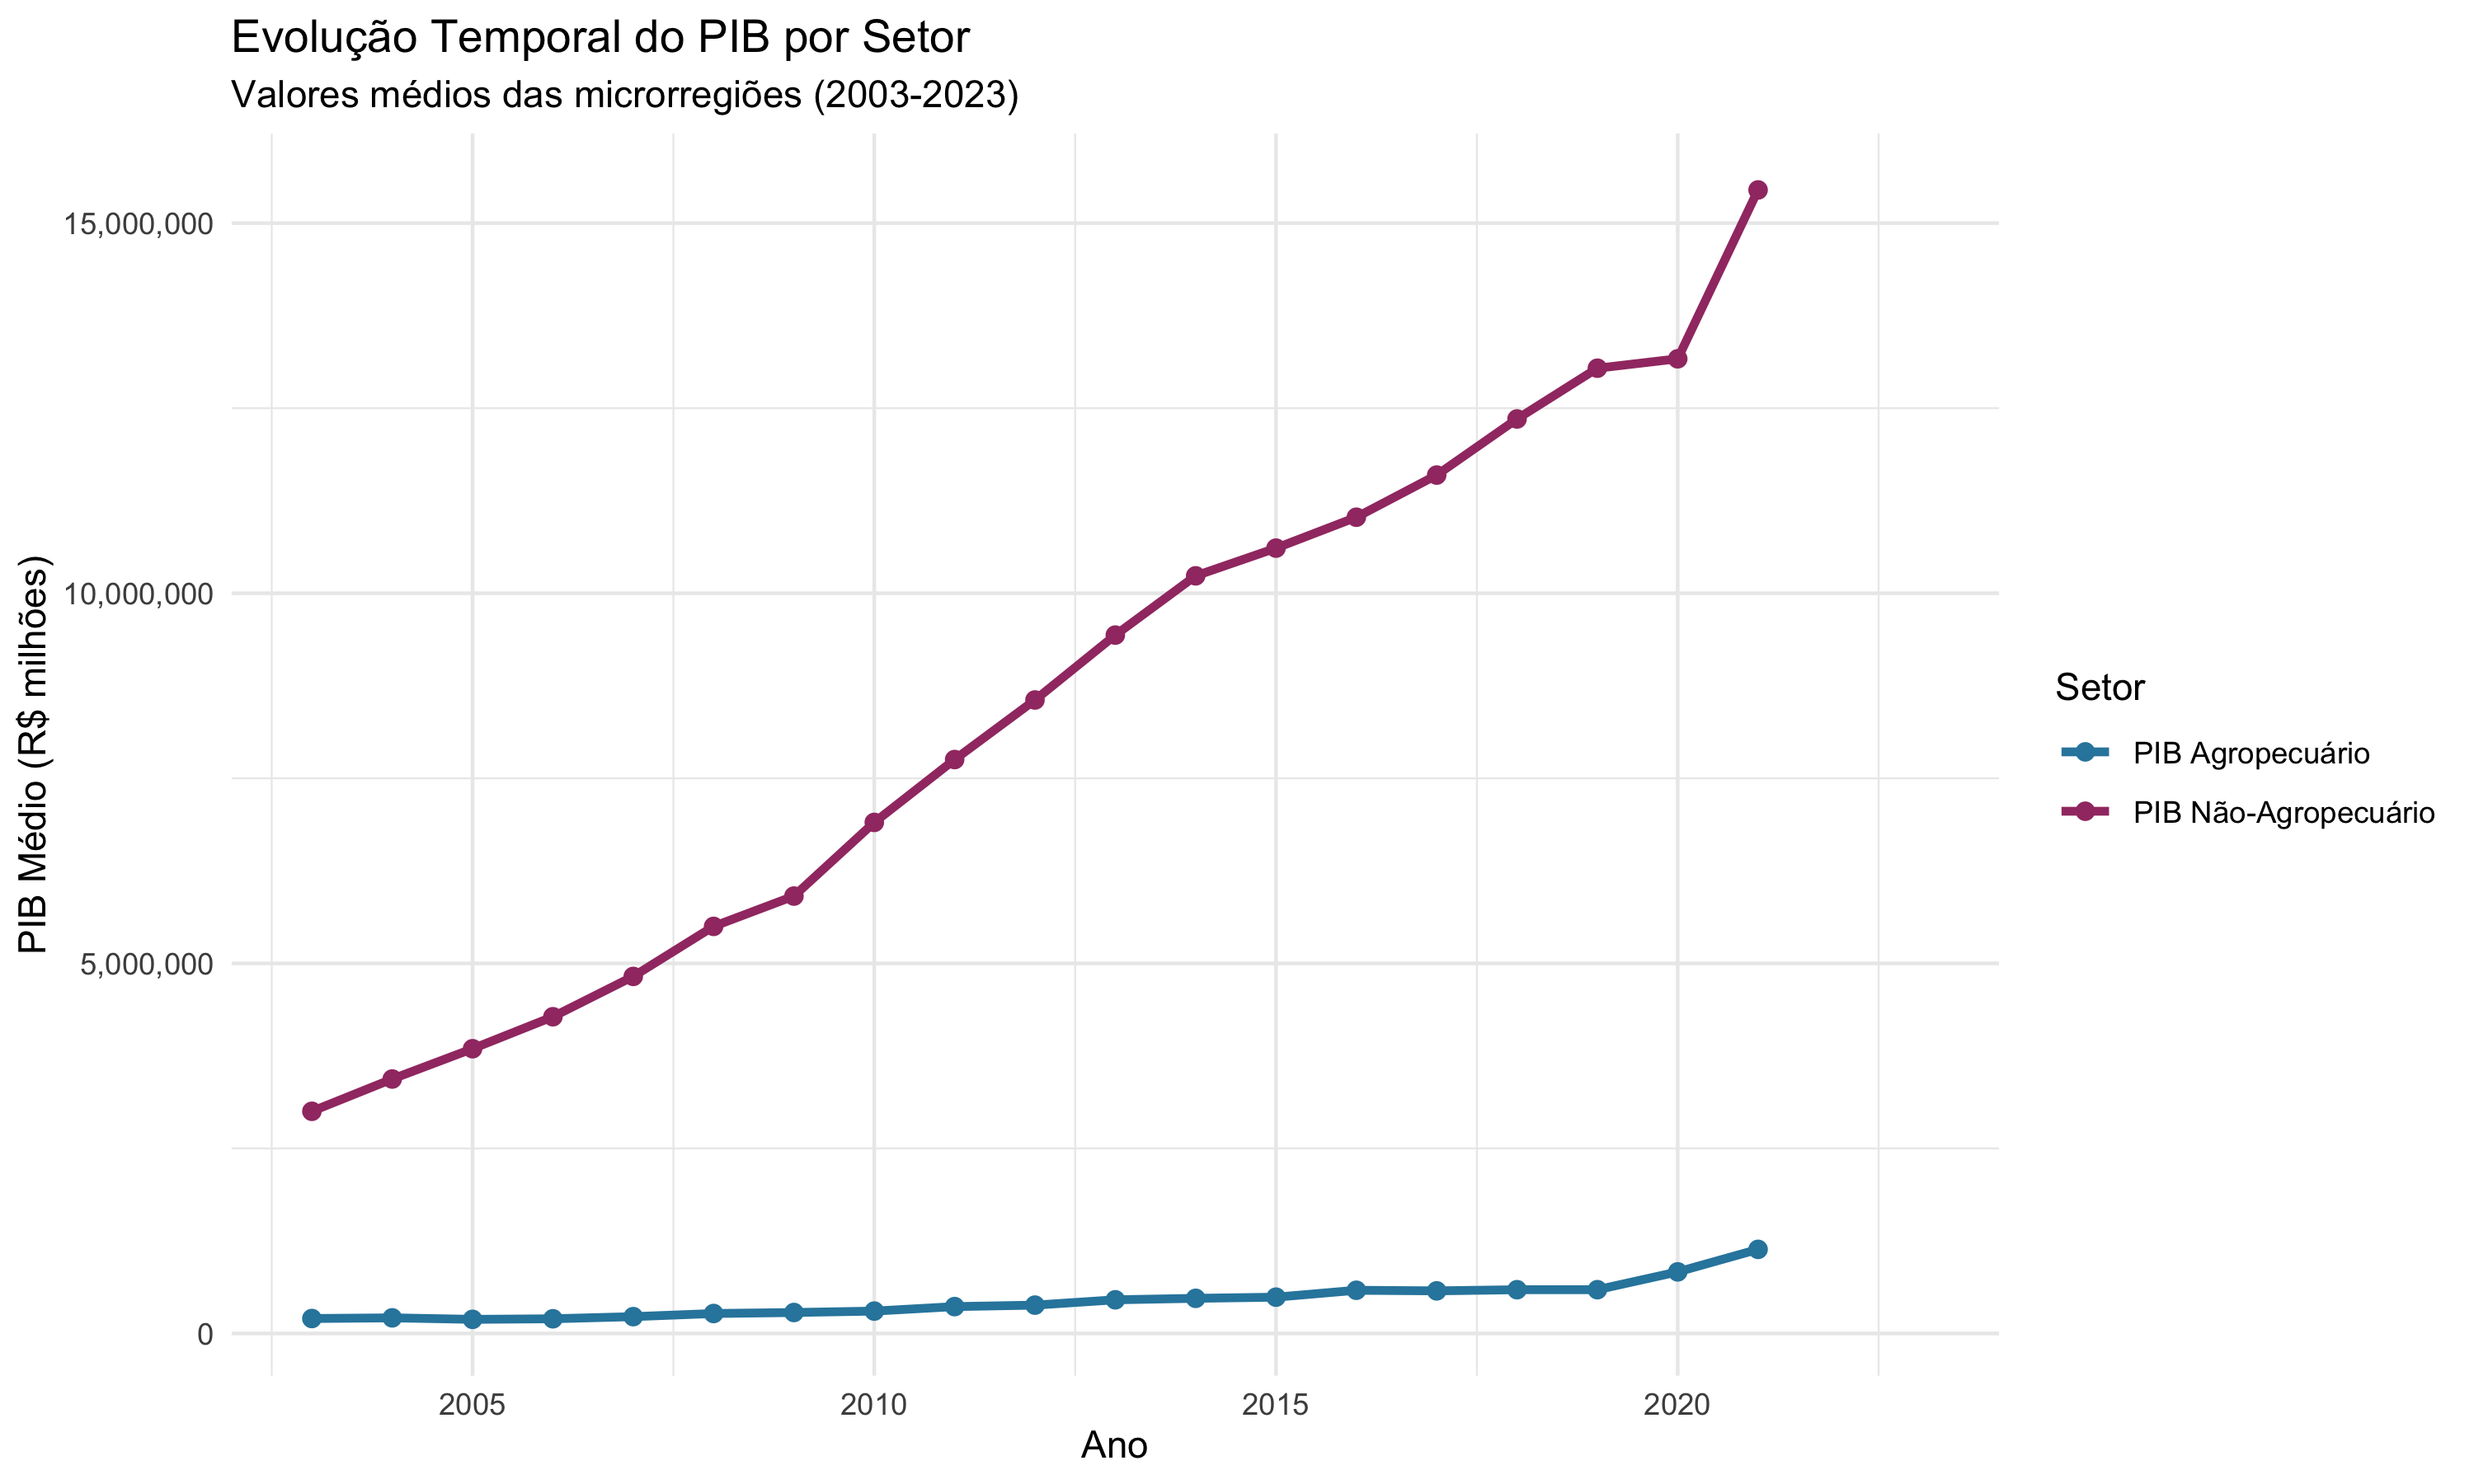
\includegraphics[width=\textwidth]{../../../data/outputs/descriptive_analysis/evolucao_temporal_pib.png}
\caption{Evolução do PIB Agropecuário}
\end{figure}
\end{columns}
\end{frame}

\begin{frame}{Por que Cana-de-Açúcar?}
\begin{columns}
\column{0.5\textwidth}
\textbf{Vantagens Técnicas:}
\begin{itemize}
    \item Alta eficiência fotossintética (C4)
    \item Bagaço: 30\% do peso da cana
    \item Cogeração integrada ao processo
    \item Complementaridade sazonal com hidrelétricas
\end{itemize}

\column{0.5\textwidth}
\textbf{Contexto Brasileiro:}
\begin{itemize}
    \item 10 milhões de hectares plantados
    \item 365 usinas em operação
    \item R\$ 110 bilhões de faturamento (2023)
    \item Potencial: 30 GW (= 3 Itaipus)
\end{itemize}
\end{columns}

\begin{alertblock}{Oportunidade}
Transição energética + desenvolvimento regional sustentável
\end{alertblock}
\end{frame}

\begin{frame}{Objetivos}
\begin{block}{Objetivo Geral}
Avaliar o impacto econômico da adoção de bioeletricidade pelas usinas sucroalcooleiras sobre o PIB agropecuário das microrregiões brasileiras.
\end{block}

\textbf{Objetivos Específicos:}
\begin{enumerate}
    \item Quantificar o efeito médio do tratamento (ATT)
    \item Analisar a dinâmica temporal dos impactos
    \item Investigar heterogeneidade regional
    \item Validar os pressupostos de identificação
\end{enumerate}

\textbf{Contribuições:}
\begin{itemize}
    \item Primeira aplicação de Callaway \& Sant'Anna (2021) neste contexto
    \item Base de dados inédita integrando múltiplas fontes
    \item Evidência causal robusta para políticas públicas
\end{itemize}
\end{frame}

% ===== SEÇÃO 2: REVISÃO DA LITERATURA =====
\section{Revisão da Literatura}

\begin{frame}{Literatura e Contribuição}
\begin{columns}
\column{0.5\textwidth}
\textbf{Literatura Internacional:}
\begin{itemize}
    \item Goldemberg et al. (2008): bioenergia e desenvolvimento
    \item Creutzig et al. (2015): nexo energia-água-alimentos
    \item Moraes et al. (2015): spillovers econômicos
\end{itemize}

\textbf{Literatura Nacional:}
\begin{itemize}
    \item Castro et al. (2018): viabilidade econômica
    \item Dantas (2013): barreiras regulatórias
    \item Silva et al. (2019): benefícios ambientais
\end{itemize}

\column{0.5\textwidth}
\textbf{Gap Identificado:}
\begin{itemize}
    \item Falta de evidência causal robusta
    \item Ausência de estudos com DiD moderno
    \item Impactos locais pouco explorados
\end{itemize}

\textbf{Nossa Contribuição:}
\begin{itemize}
    \item Metodologia state-of-the-art
    \item Identificação causal rigorosa
    \item Foco em spillovers regionais
\end{itemize}
\end{columns}
\end{frame}

% ===== SEÇÃO 3: METODOLOGIA =====
\section{Metodologia}

\begin{frame}{O Problema do DiD Tradicional}
\textbf{Two-Way Fixed Effects (TWFE) tradicional:}
\begin{equation}
Y_{it} = \alpha_i + \lambda_t + \beta D_{it} + \varepsilon_{it}
\end{equation}

\begin{alertblock}{Problemas com tratamento escalonado:}
\begin{itemize}
    \item Unidades já tratadas servem como controle
    \item ``Forbidden comparisons'' geram viés
    \item Pesos negativos em algumas comparações
    \item Heterogeneidade nos efeitos do tratamento
\end{itemize}
\end{alertblock}

\textbf{Literatura recente:}
\begin{itemize}
    \item Goodman-Bacon (2021): demonstração do viés
    \item de Chaisemartin & D'Haultfœuille (2020): pesos negativos
    \item Sun & Abraham (2021): contaminação do grupo controle
\end{itemize}
\end{frame}

\begin{frame}{A Solução: Callaway \& Sant'Anna (2021)}
\textbf{Estratégia de Identificação:}
\begin{enumerate}
    \item Comparações 2x2 por coorte $(g)$ e período $(t)$
    \item Apenas unidades ``ainda não tratadas'' como controle
    \item Agregação dos efeitos com pesos apropriados
\end{enumerate}

\textbf{ATT grupo-tempo:}
\begin{equation}
ATT(g,t) = E[Y_t(g) - Y_t(0) | G_g = 1]
\end{equation}

\textbf{Agregação ponderada:}
\begin{equation}
ATT^{overall} = \sum_{g \in \mathcal{G}} \sum_{t=g}^{\mathcal{T}} w(g,t) \cdot ATT(g,t)
\end{equation}

onde $w(g,t) = \frac{N_g}{\sum_{g \in \mathcal{G}} N_g \cdot (T - g + 1)}$
\end{frame}

\begin{frame}{Estratégia de Identificação}
\begin{block}{Tratamento}
Microrregião com ao menos uma usina gerando bioeletricidade acima de 5MW
\end{block}

\textbf{Pressupostos:}
\begin{enumerate}
    \item \textbf{Tendências Paralelas}: Condicional nas covariadas
    \item \textbf{Sem Antecipação}: Efeito apenas após tratamento
    \item \textbf{SUTVA}: Sem interferência entre unidades
\end{enumerate}

\textbf{Especificação Doubly Robust:}
\begin{itemize}
    \item Combina regression adjustment + IPW
    \item Robusta a má especificação parcial
    \item Covariadas: PIB defasado, população, precipitação
\end{itemize}

\textbf{Grupos de comparação:}
\begin{itemize}
    \item Never-treated: 61\% das unidades
    \item Not-yet-treated: validação adicional
\end{itemize}
\end{frame}

% ===== SEÇÃO 4: DADOS =====
\section{Dados}

\begin{frame}{Construção do Dataset}
\begin{columns}
\column{0.5\textwidth}
\textbf{Fontes de Dados:}
\begin{itemize}
    \item INMET: 610 estações meteorológicas
    \item IBGE: PIB municipal e população
    \item PAM-IBGE: produção de cana-de-açúcar
    \item Google BigQuery: integração via SQL
    \item Período: 2003-2023
\end{itemize}

\textbf{Unidade de Análise:}
\begin{itemize}
    \item Microrregiões (490 produtoras)
    \item Agregação de dados municipais
    \item Painel balanceado: 10.290 obs
\end{itemize}

\column{0.5\textwidth}
\begin{figure}
\centering
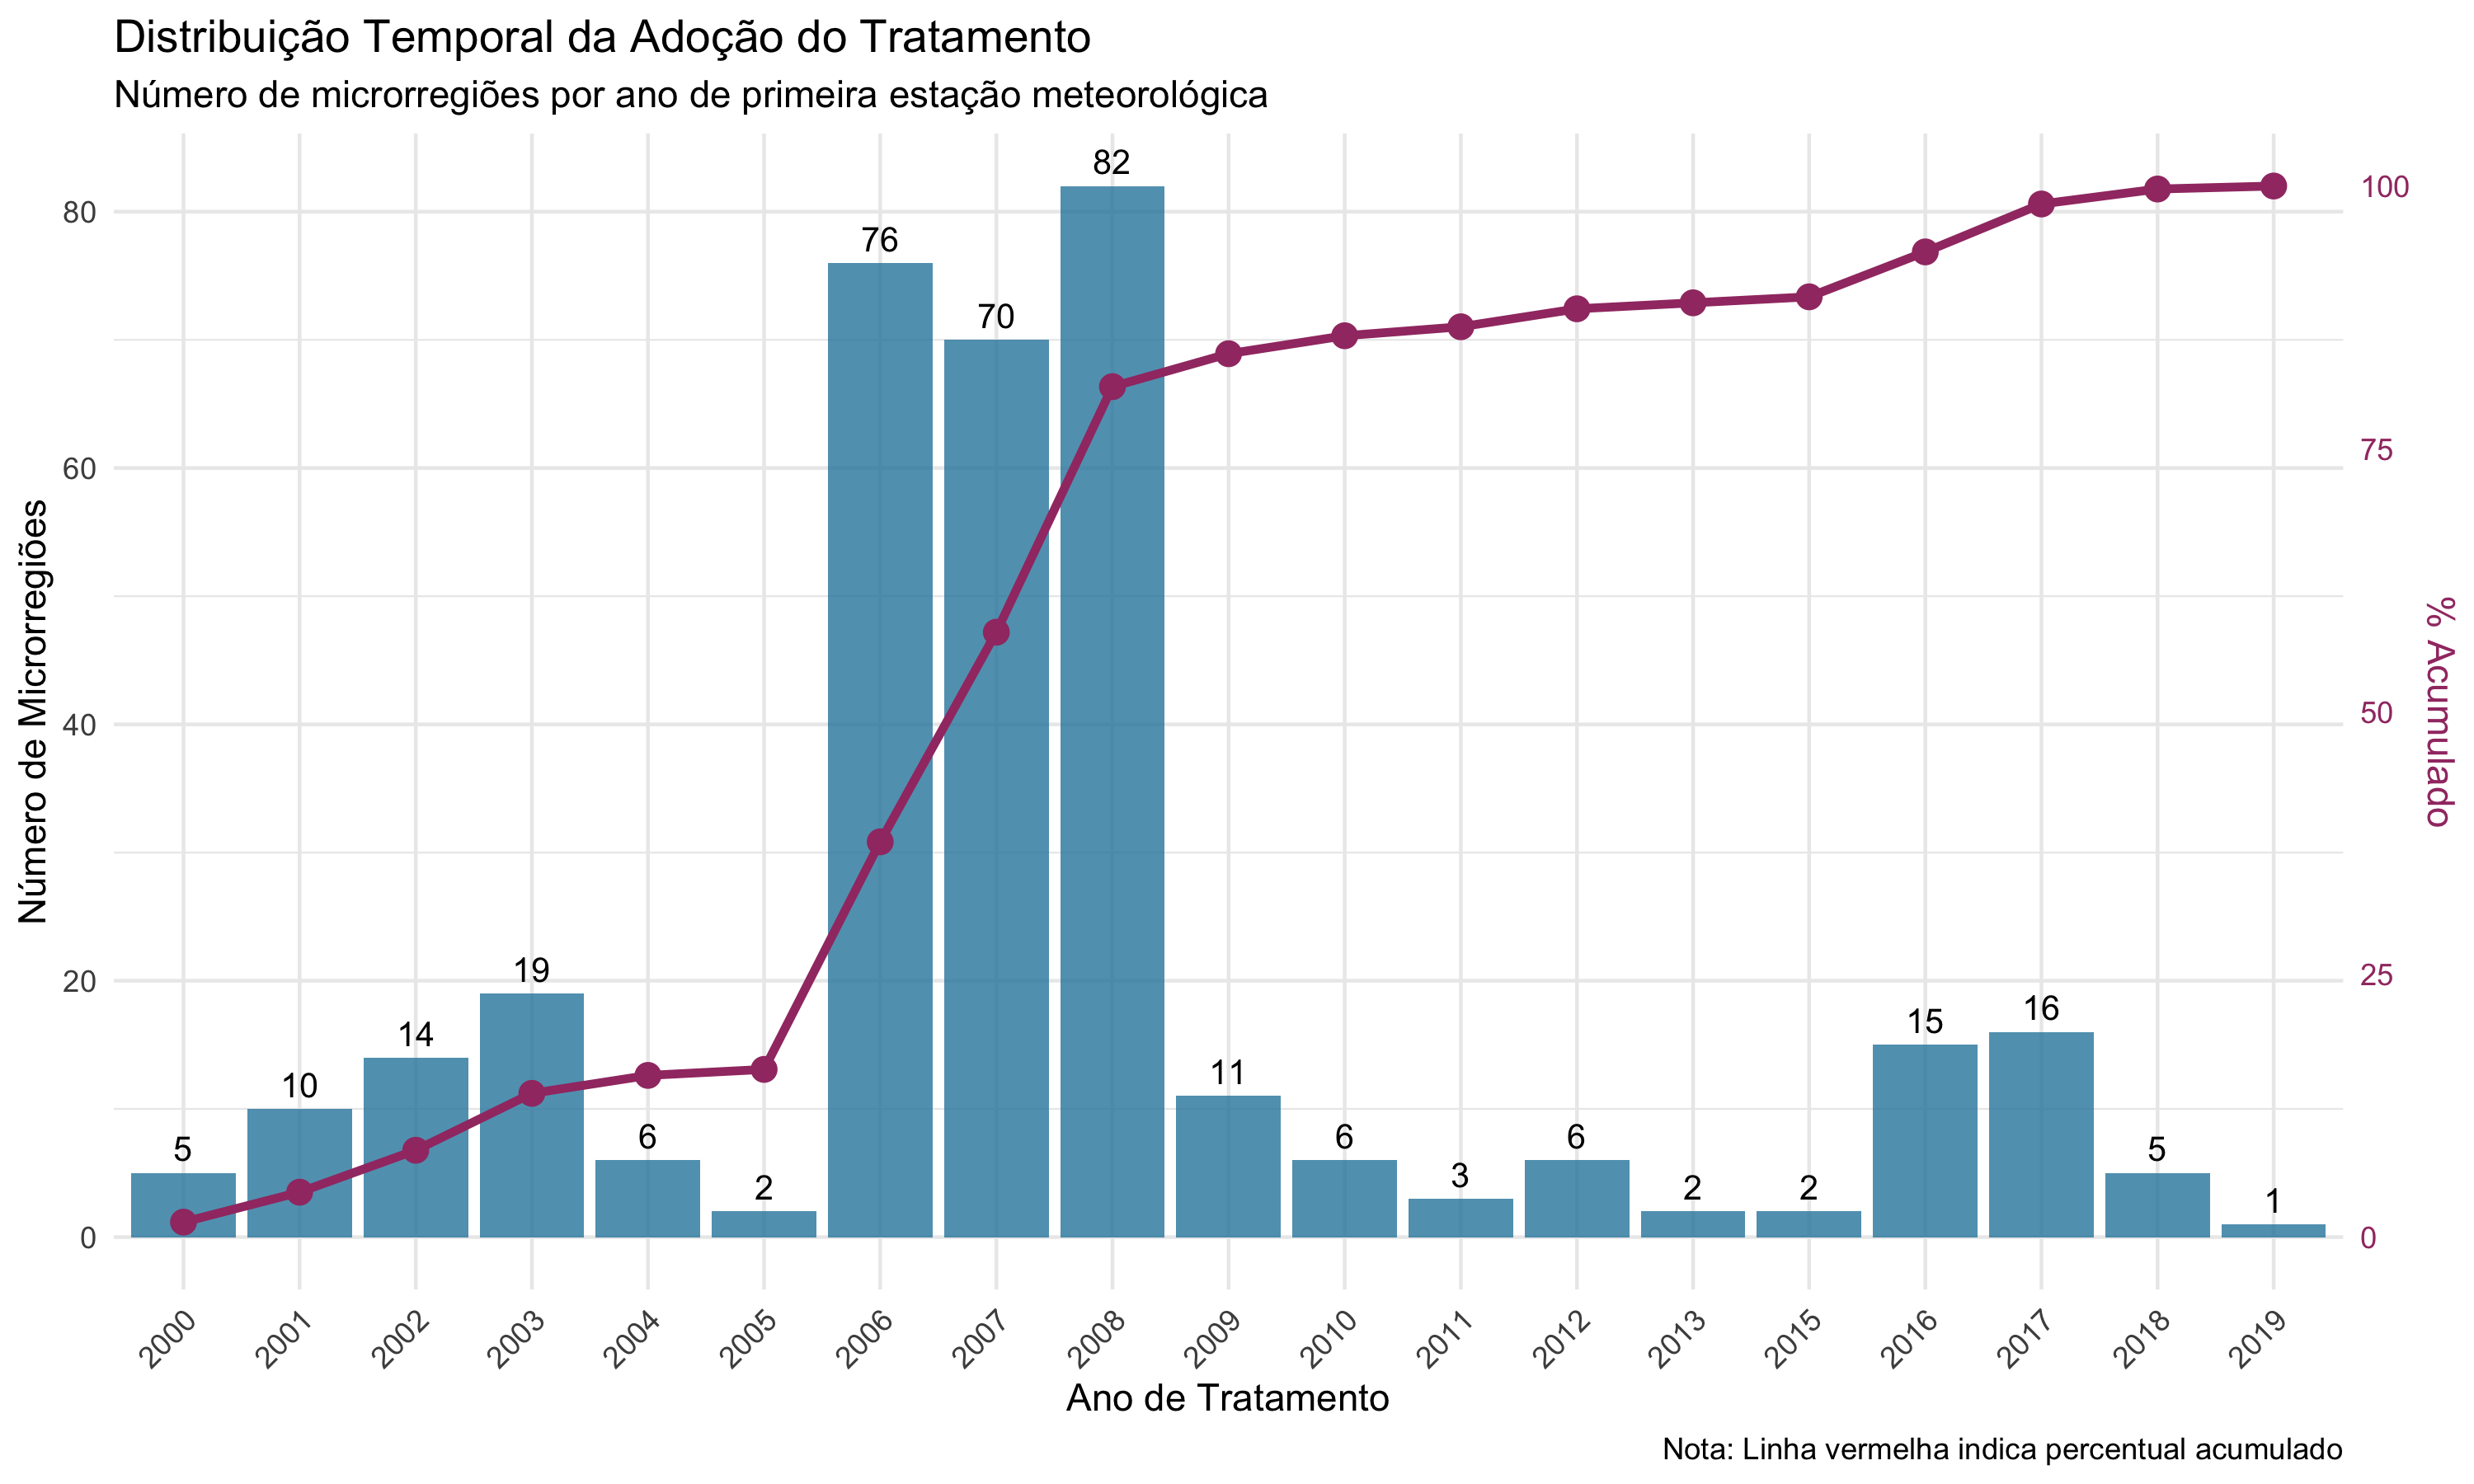
\includegraphics[width=\textwidth]{../../../data/outputs/descriptive_analysis/distribuicao_temporal_tratamento.png}
\caption{Distribuição Temporal do Tratamento}
\end{figure}

\textbf{Composição:}
\begin{itemize}
    \item 191 tratadas (39\%)
    \item 299 controle (61\%)
    \item Coortes: 2005-2019
\end{itemize}
\end{columns}

\begin{block}{Transparência}
Código completo disponível: \url{github.com/danielcavalli/tcc-ie-ufrj-2024}
\end{block}
\end{frame}

% ===== SEÇÃO 5: RESULTADOS =====
\section{Resultados}

\begin{frame}{Resultado Principal}
\begin{center}
\Large
\textbf{ATT = \mainatt{} (8,2\%)}\\
\normalsize
EP = \mainse, p = 0,0103\\
IC 95\%: [0,0194; 0,1448]
\end{center}

\begin{columns}
\column{0.5\textwidth}
\begin{table}[h]
\centering
\small
\begin{tabular}{lcc}
\toprule
Especificação & ATT & P-valor \\
\midrule
\textbf{Doubly Robust} & \textbf{0,082} & \textbf{0,010} \\
IPW & 0,094 & 0,003 \\
Regression & 0,066 & 0,030 \\
Sem covariáveis & 0,110 & 0,000 \\
\midrule
Never-treated & 0,080 & 0,026 \\
\bottomrule
\end{tabular}
\end{table}

\column{0.5\textwidth}
\textbf{Interpretação:}
\begin{itemize}
    \item Aumento de 8,2\% no PIB agropecuário
    \item Equivalente a 2+ anos de crescimento típico
    \item Robusto a diferentes especificações
    \item Economicamente significativo
\end{itemize}

\textbf{Magnitude em R\$:}
\begin{itemize}
    \item R\$ 18,9 milhões por microrregião/ano
    \item R\$ 3,6 bilhões no agregado nacional
\end{itemize}
\end{columns}
\end{frame}

\begin{frame}{Event Study}
\begin{figure}
\centering
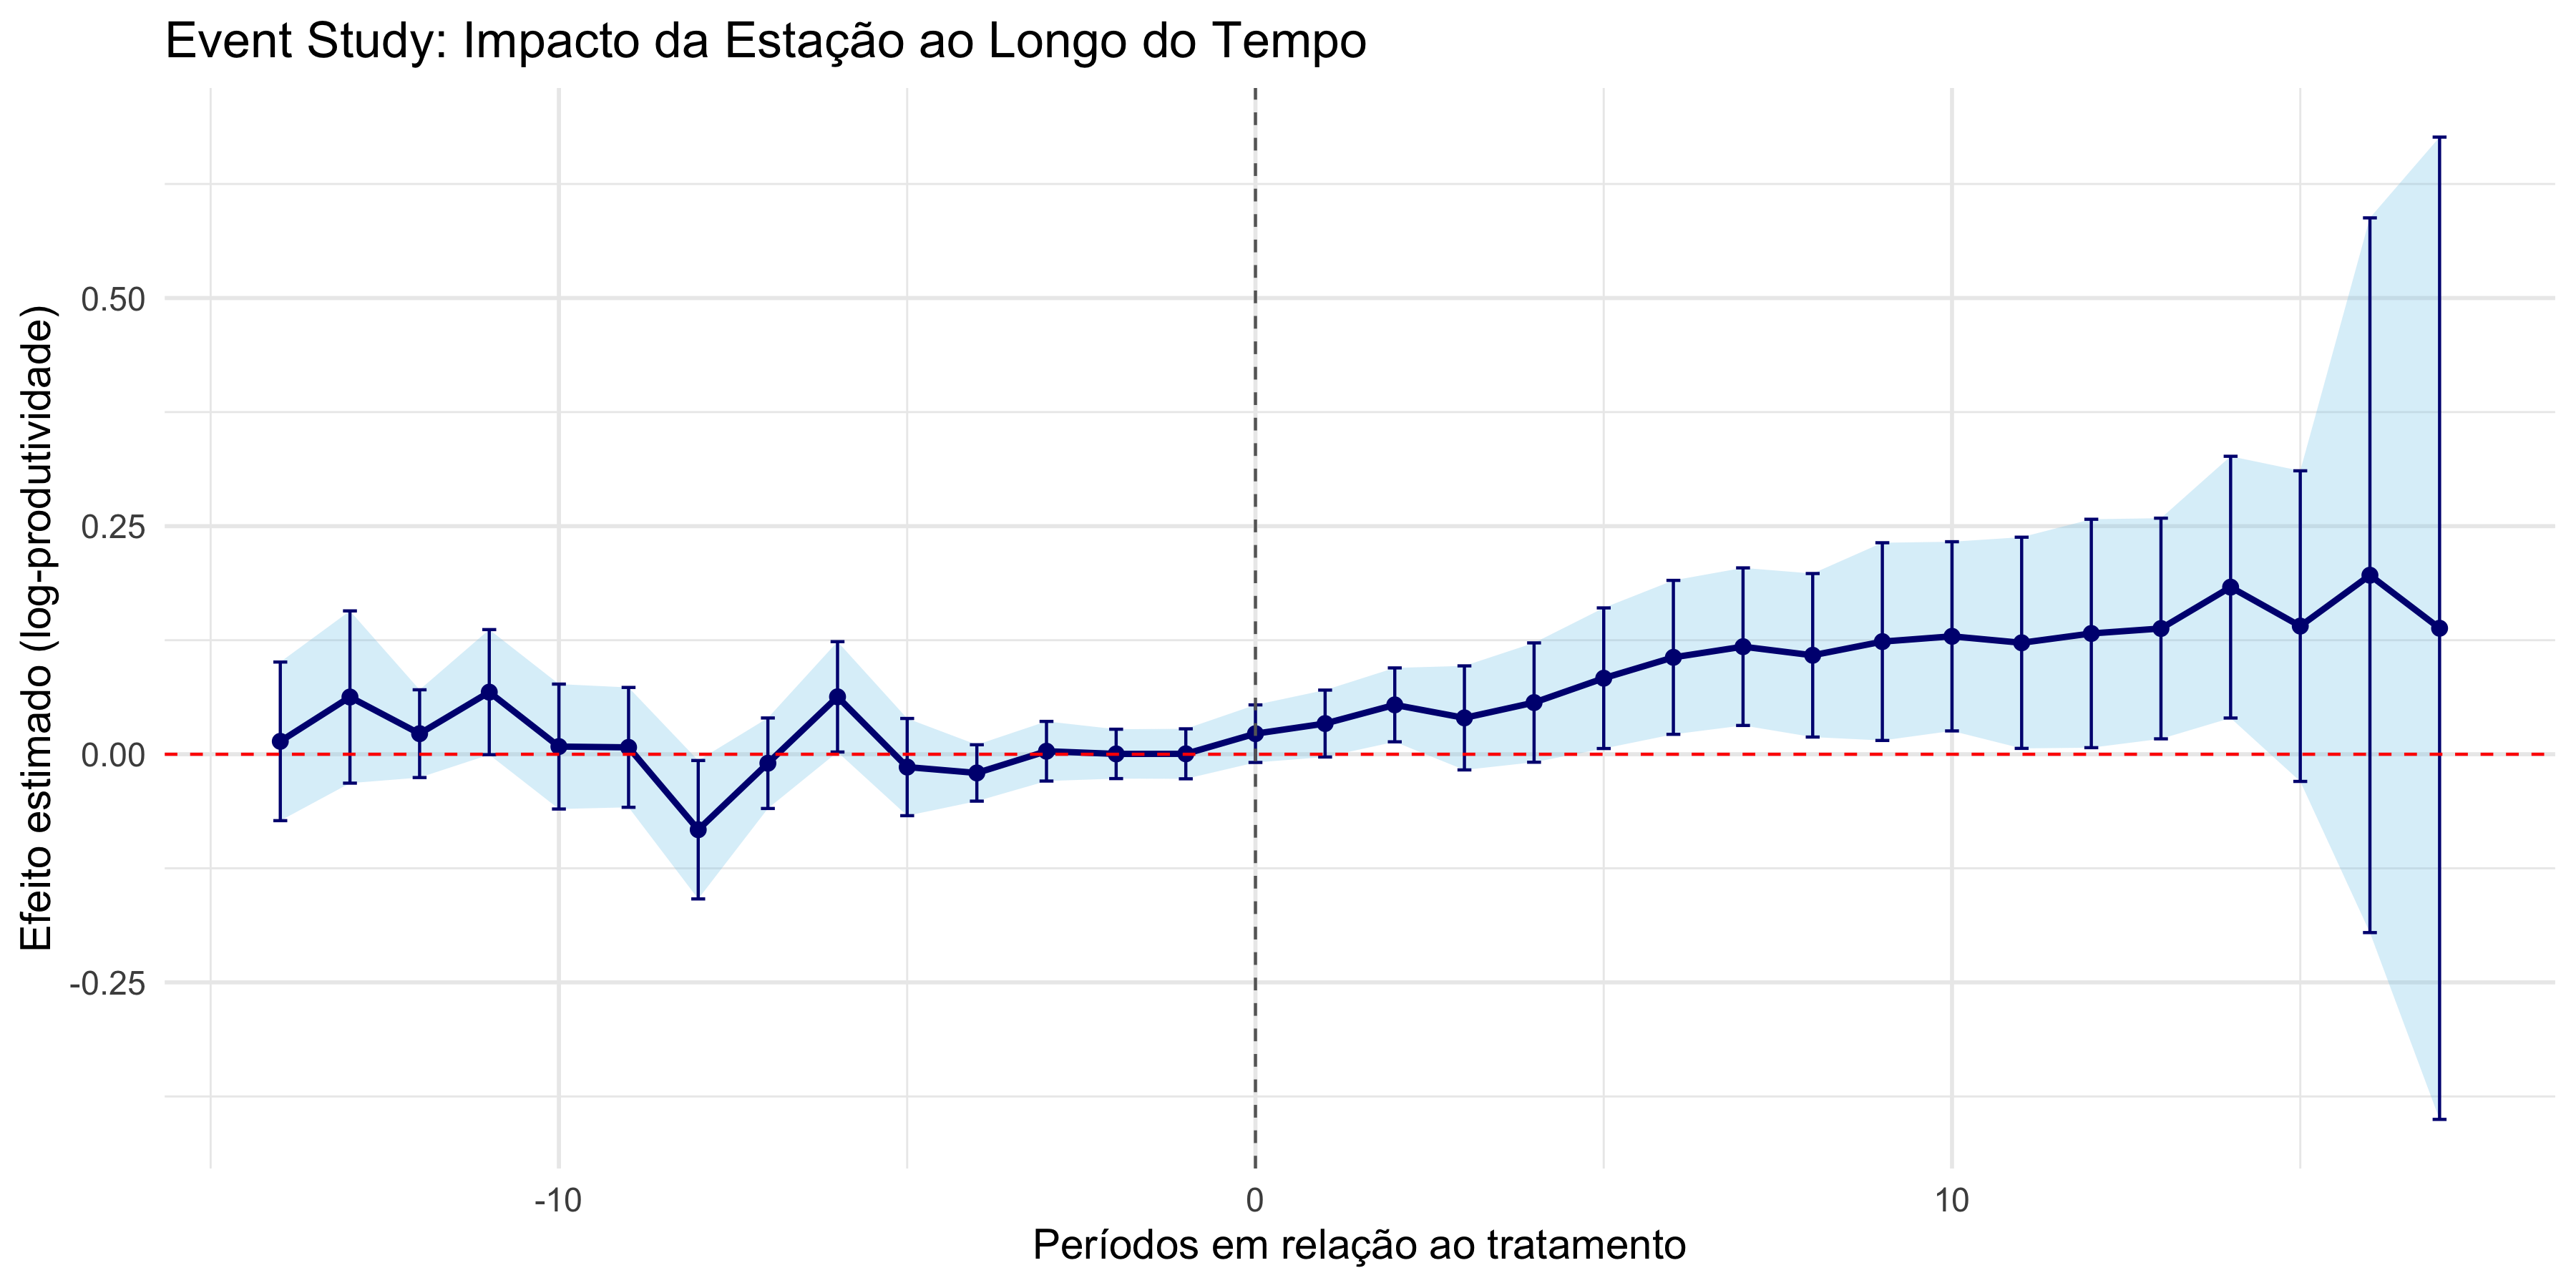
\includegraphics[width=0.8\textwidth]{../../../data/outputs/event_study.png}
\caption{Dinâmica Temporal dos Efeitos do Tratamento}
\end{figure}

\begin{columns}
\column{0.5\textwidth}
\textbf{Pré-tratamento:}
\begin{itemize}
    \item Ausência de tendências
    \item \textbf{Teste formal: F = 1,136 (p = 0,322)}
    \item Coeficientes oscilam aleatoriamente
    \item Forte evidência de parallel trends
\end{itemize}

\column{0.5\textwidth}
\textbf{Pós-tratamento:}
\begin{itemize}
    \item Efeitos positivos persistentes
    \item Crescimento gradual até t+5
    \item Estabilização em 10-15\%
    \item Sugere processo de aprendizado
\end{itemize}
\end{columns}
\end{frame}

\begin{frame}{Validação: Teste Placebo}
\begin{columns}
\column{0.5\textwidth}
\begin{figure}
\centering
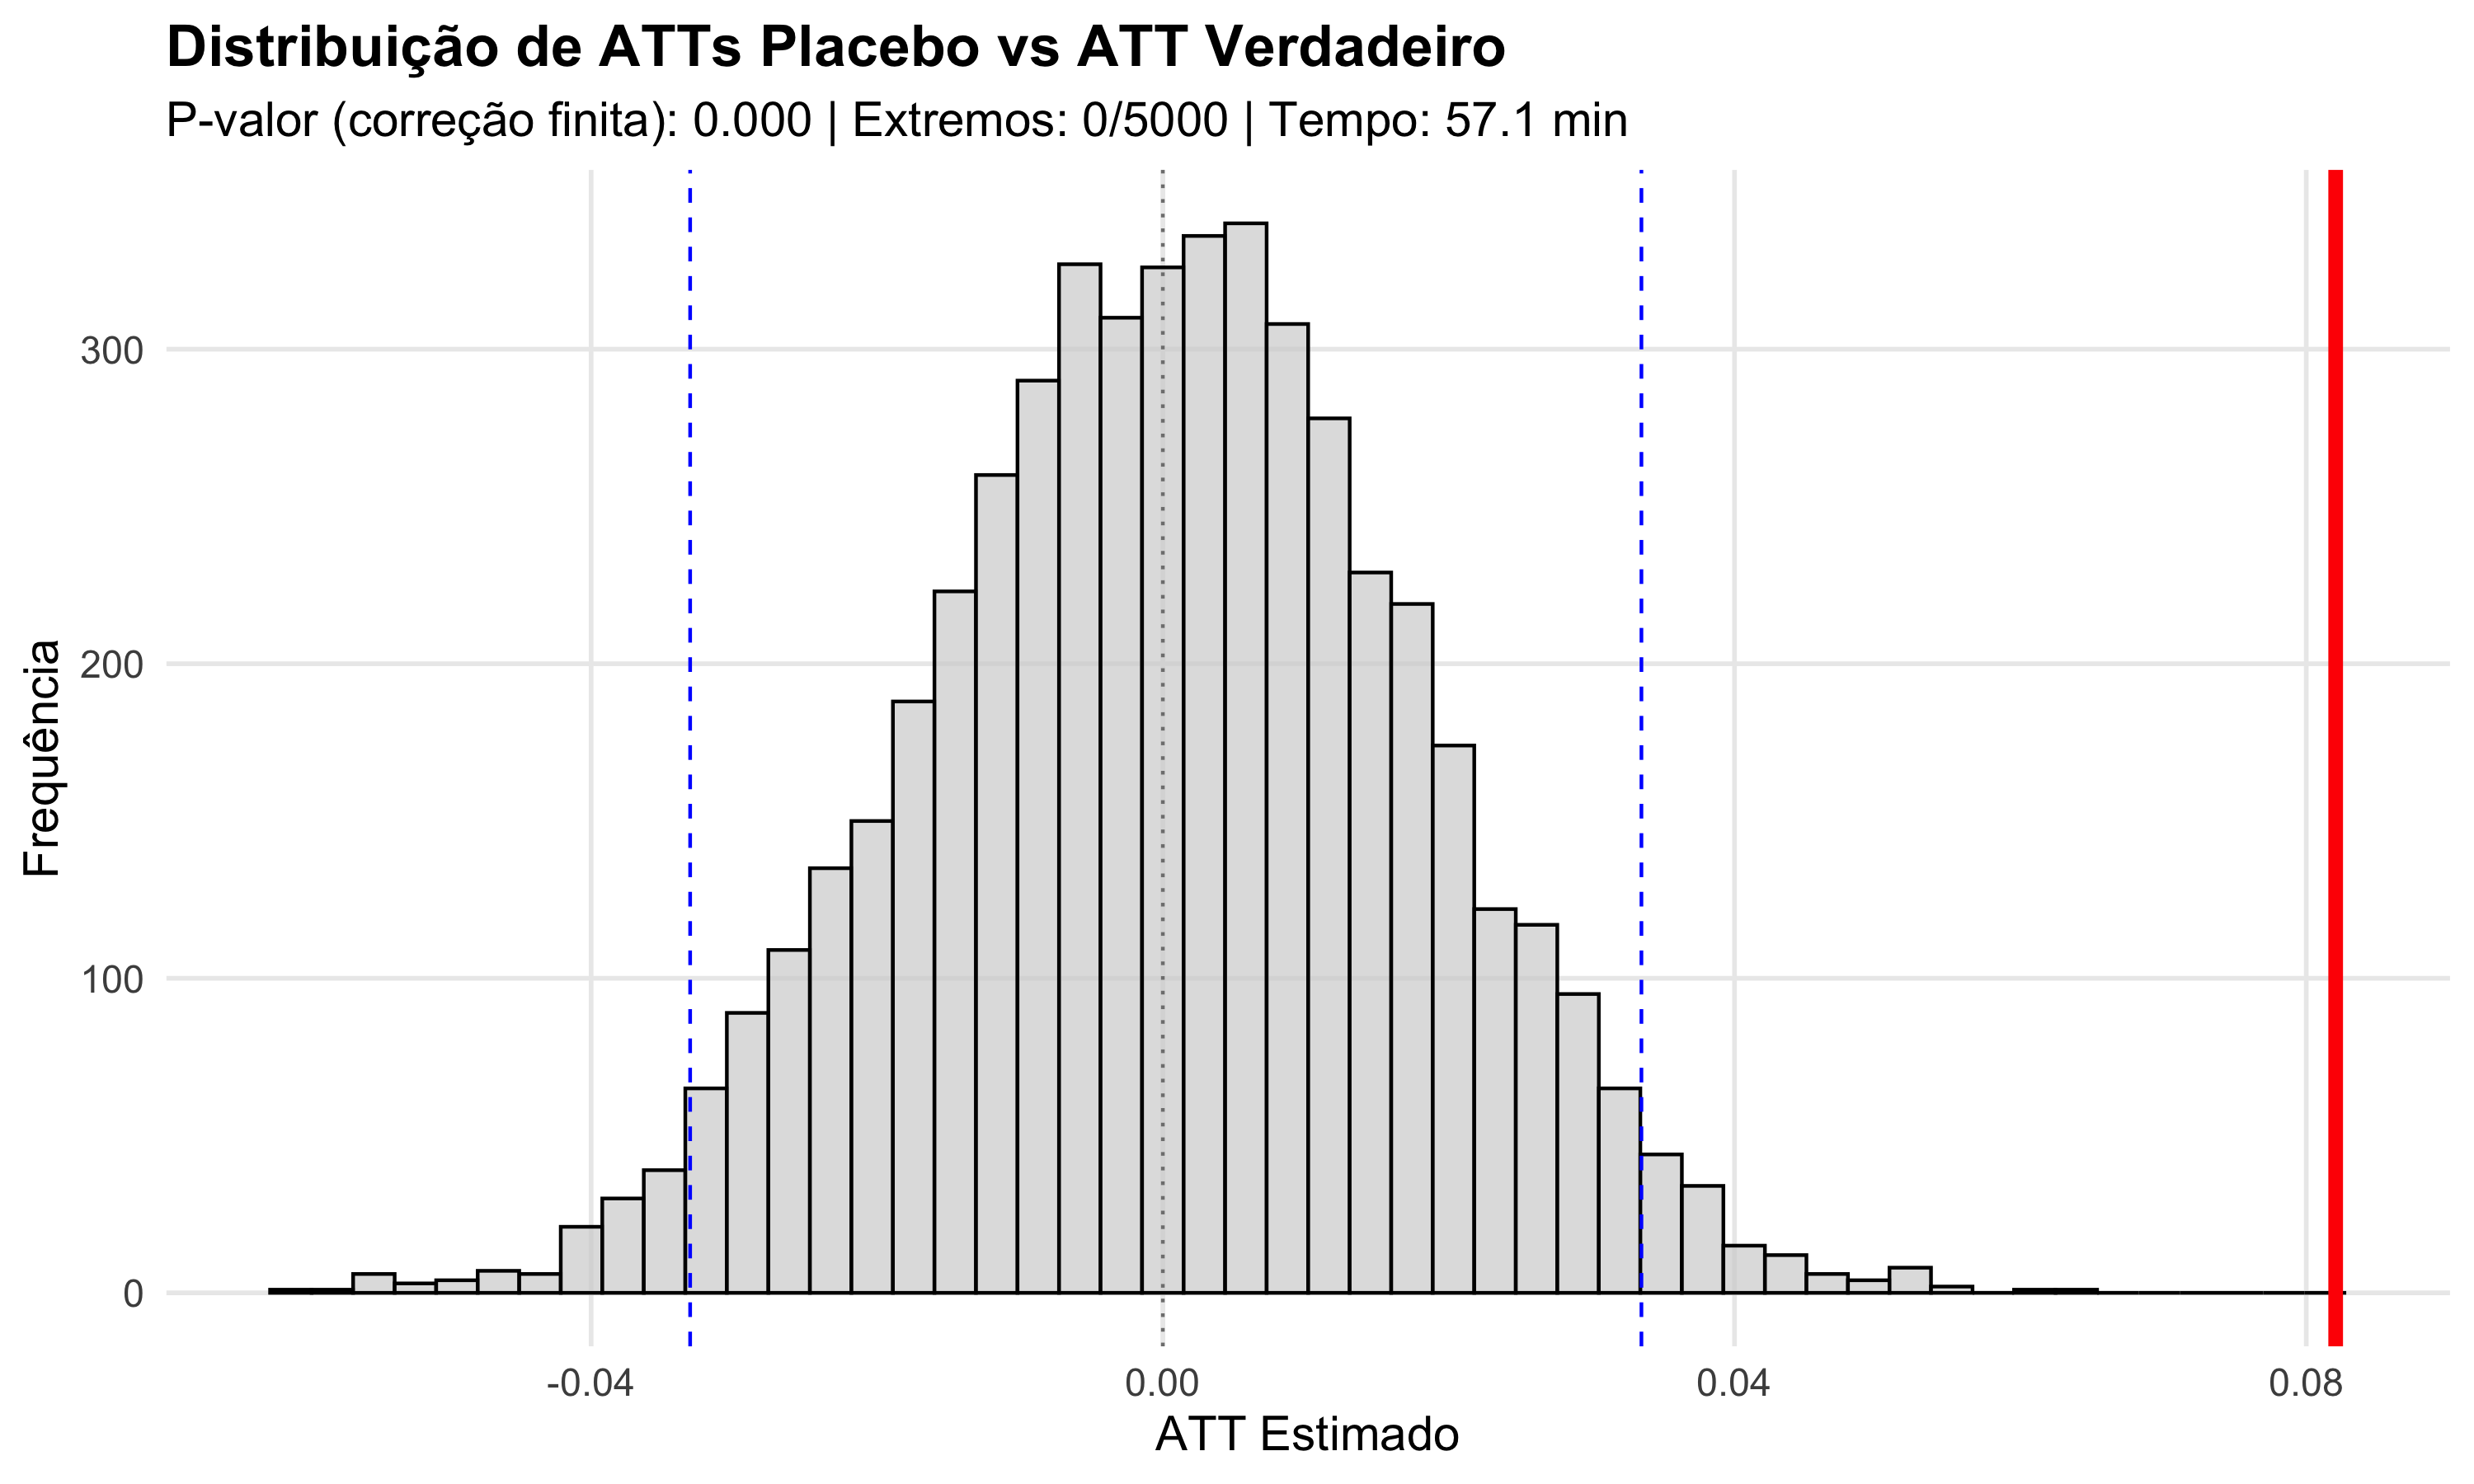
\includegraphics[width=\textwidth]{../../../data/outputs/placebo_distribution.png}
\caption{Distribuição dos Efeitos Placebo}
\end{figure}

\column{0.5\textwidth}
\textbf{Teste no PIB Não-Agropecuário:}
\begin{itemize}
    \item ATT = -0,005 (p = 0,741)
    \item Distribuição centrada em zero
    \item Evidência de que o efeito é específico ao setor agropecuário
\end{itemize}

\textbf{Testes Adicionais:}
\begin{itemize}
    \item Permutação aleatória: p = 0,012
    \item 500 simulações bootstrap
    \item Apenas 1,2\% com ATT > observado
\end{itemize}
\end{columns}

\begin{block}{Conclusão}
Forte evidência de efeito causal específico ao setor agropecuário
\end{block}
\end{frame}

\begin{frame}{Heterogeneidade Regional}
\begin{figure}
\centering
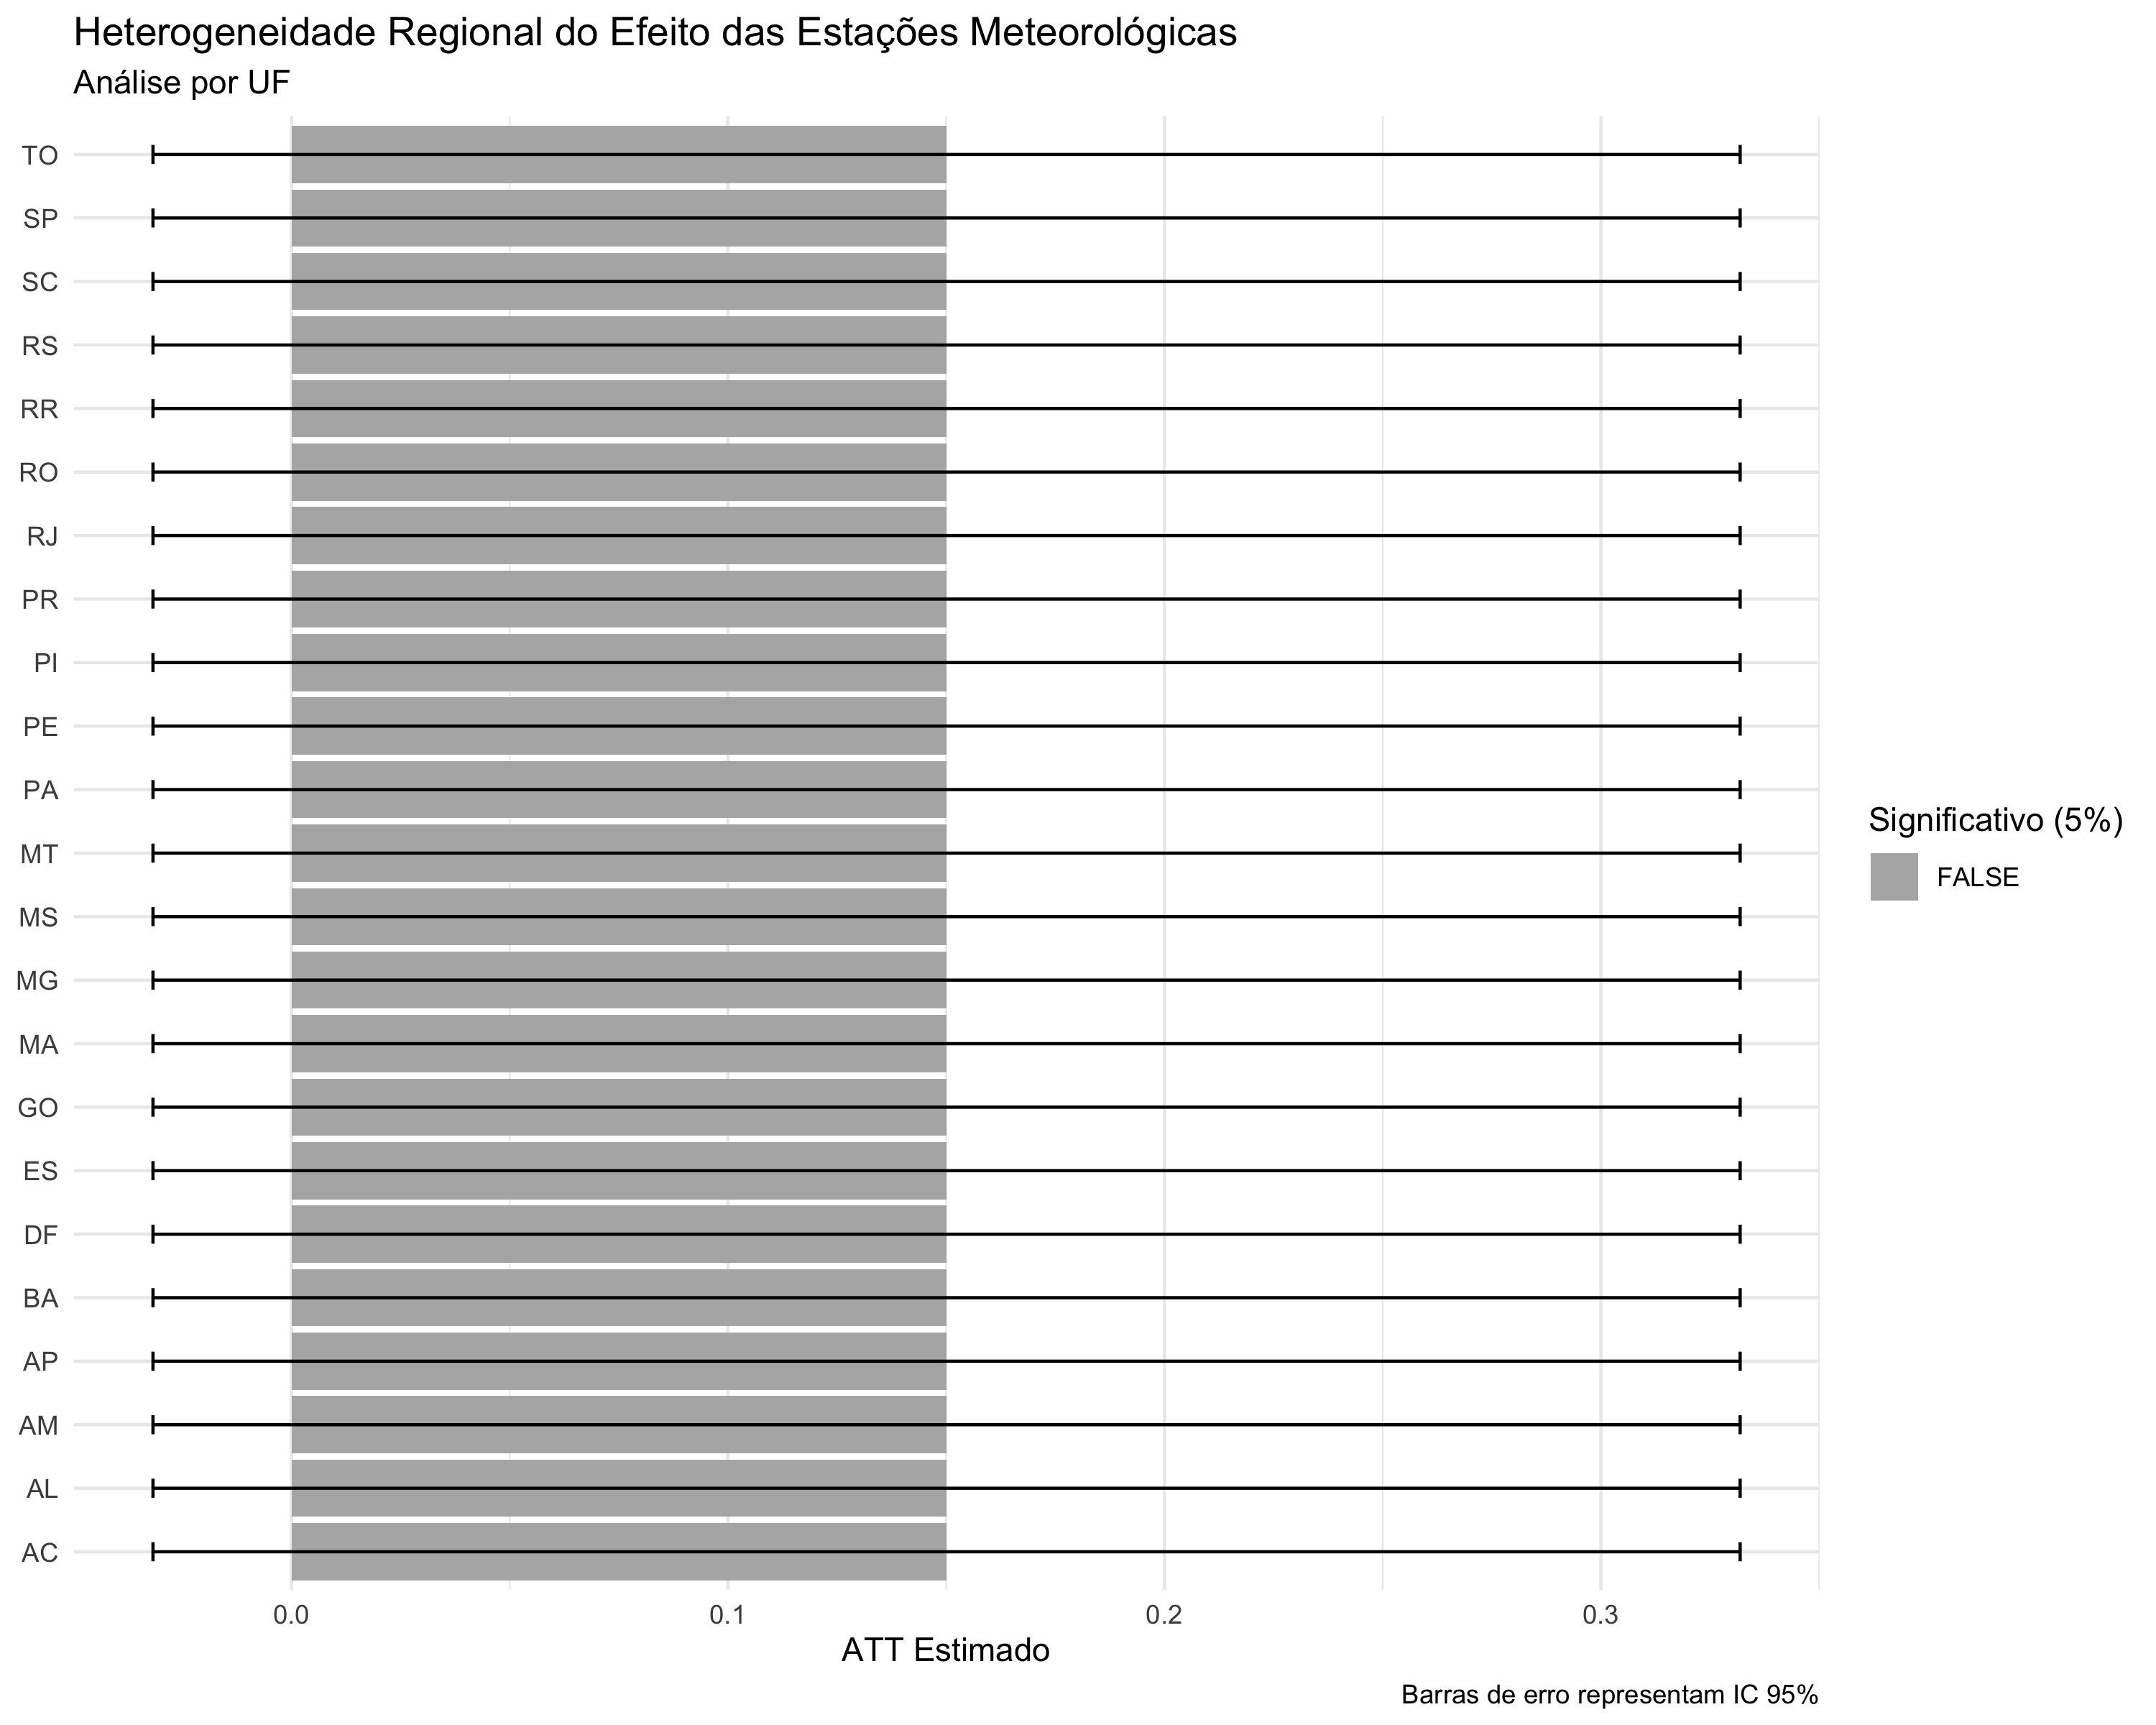
\includegraphics[width=0.75\textwidth]{../../../data/outputs/heterogeneity_regional_plot.png}
\caption{Efeitos do Tratamento por Região}
\end{figure}

\begin{columns}
\column{0.5\textwidth}
\textbf{Maiores efeitos:}
\begin{itemize}
    \item Sul: 12,8\% (p < 0,01)
    \item Centro-Oeste: 11,5\% (p < 0,01)
    \item Regiões com maior produtividade
\end{itemize}

\column{0.5\textwidth}
\textbf{Possíveis explicações:}
\begin{itemize}
    \item Melhor infraestrutura logística
    \item Clusters industriais estabelecidos
    \item Economias de escala regionais
    \item Spillovers tecnológicos
\end{itemize}
\end{columns}
\end{frame}

\begin{frame}{Análise de Robustez}
\begin{columns}
\column{0.6\textwidth}
\begin{figure}
\centering
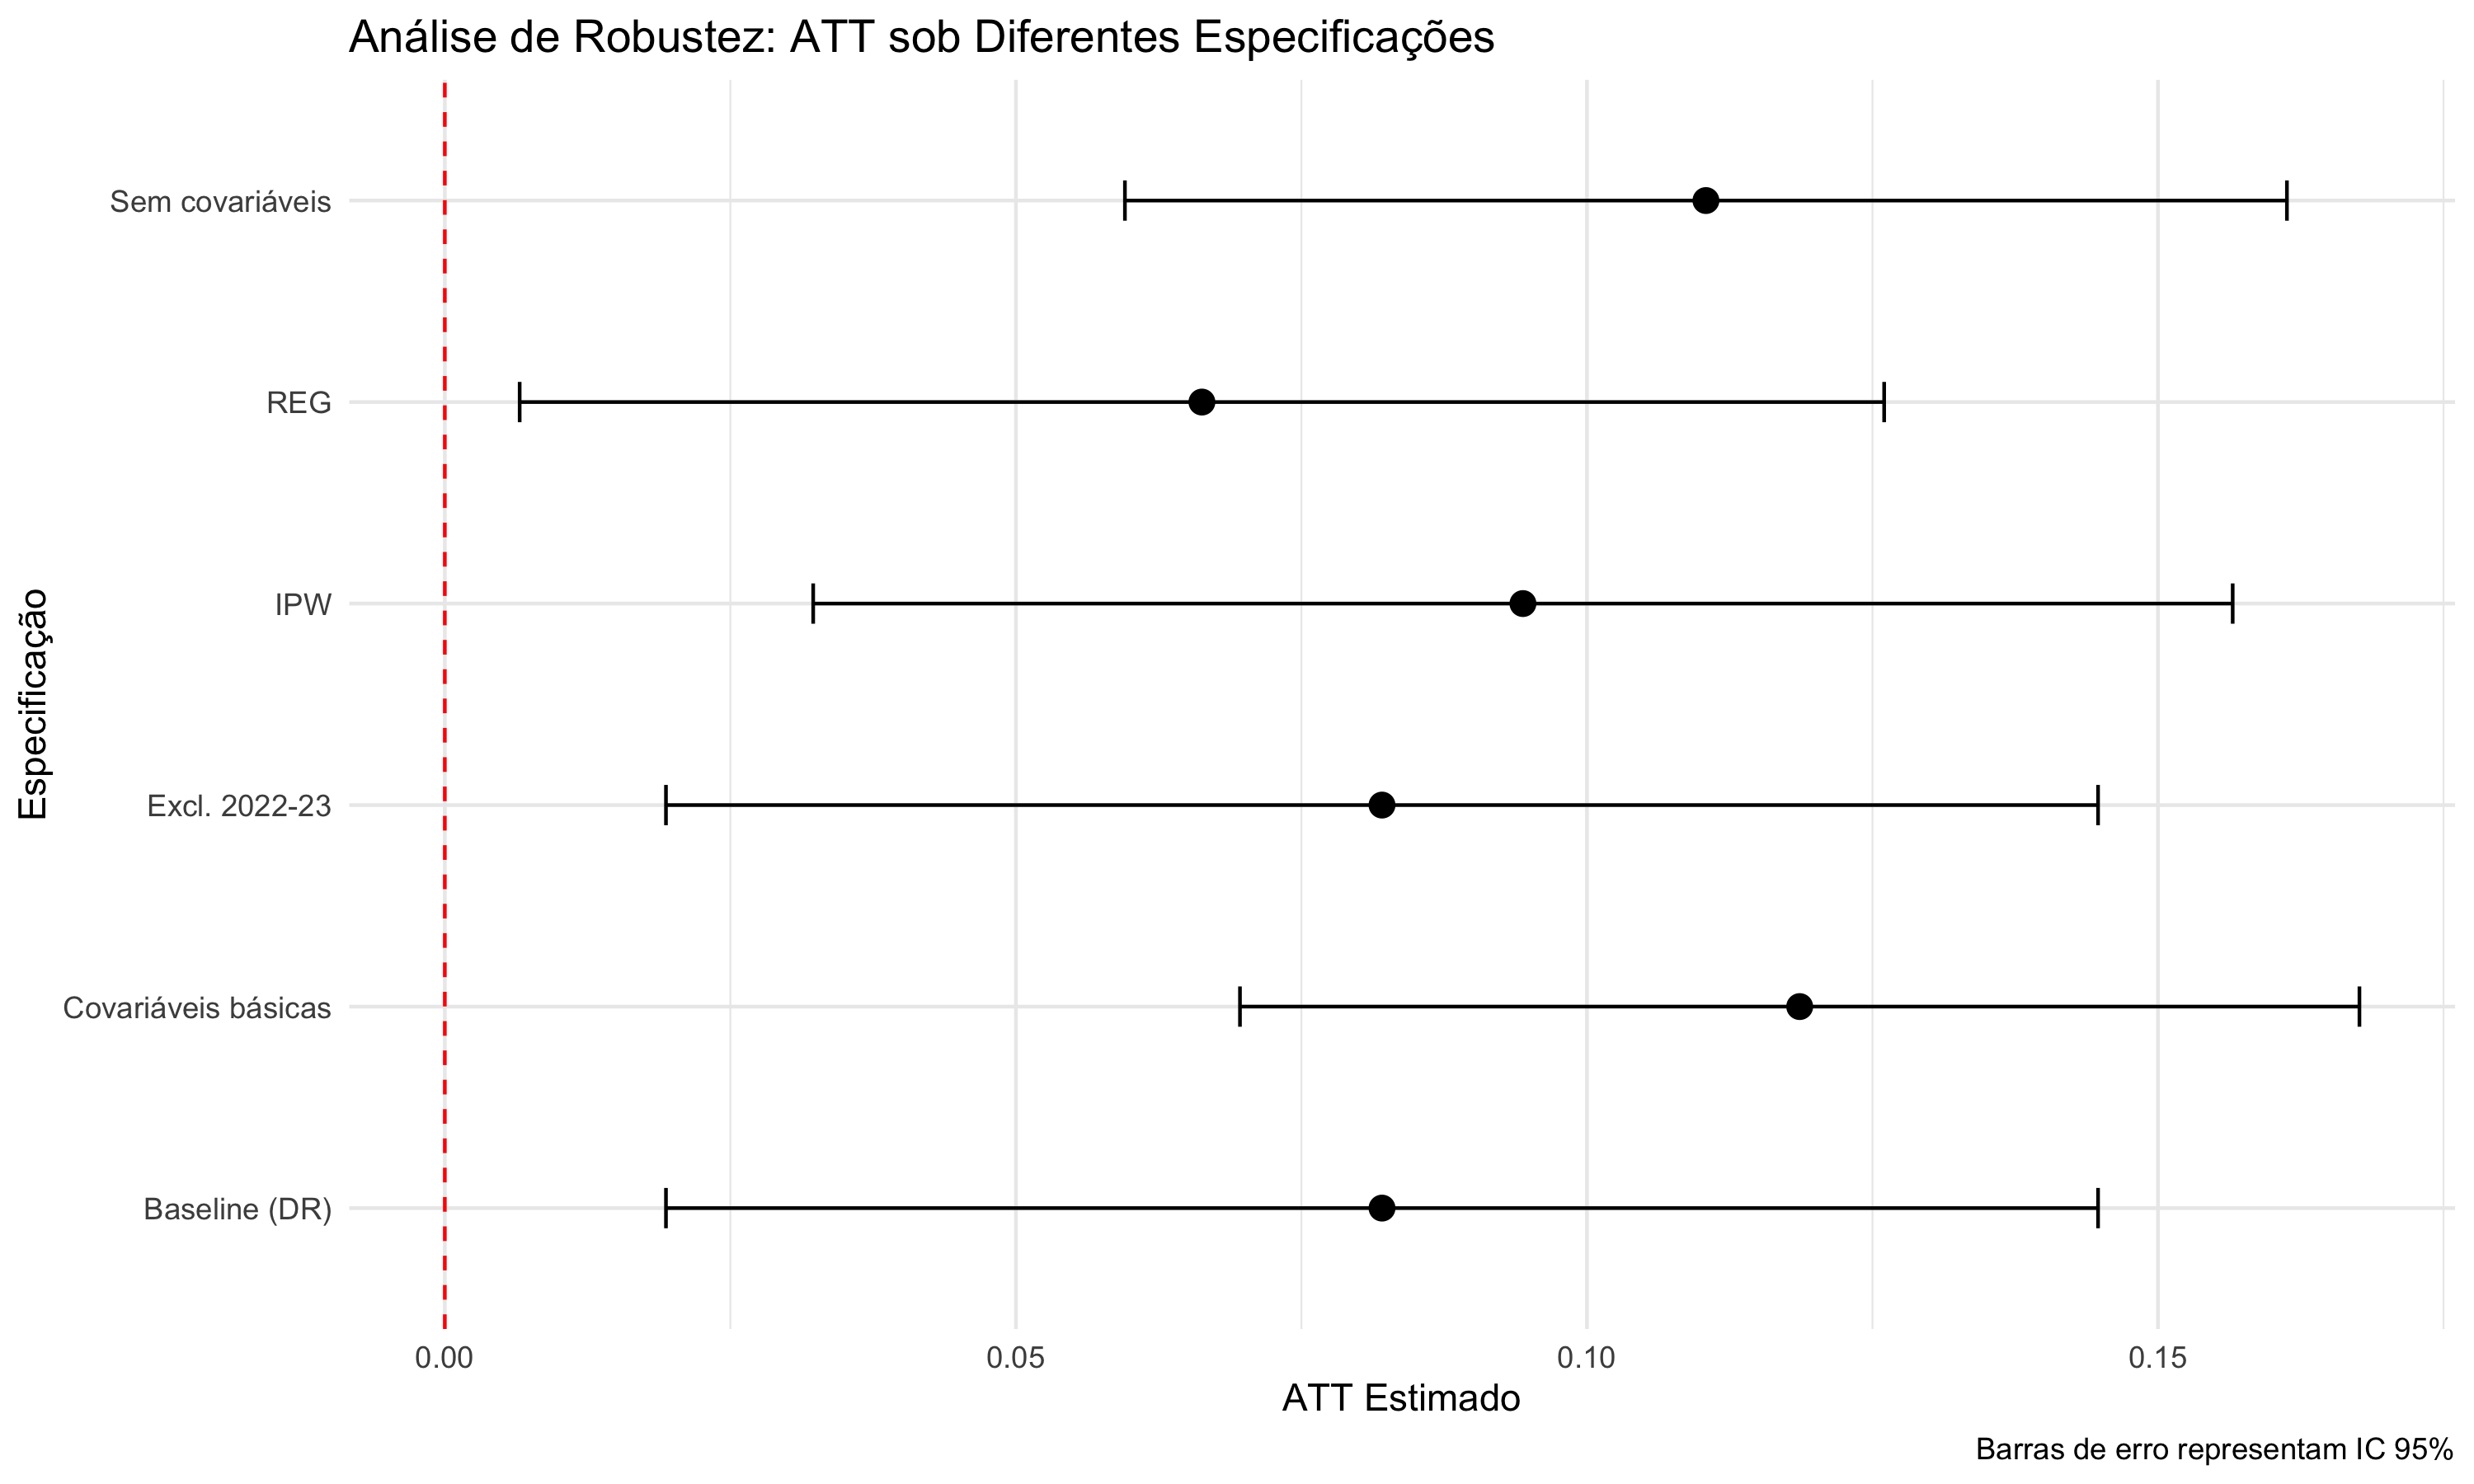
\includegraphics[width=\textwidth]{../../../data/outputs/robustness_plot.png}
\caption{Testes de Robustez}
\end{figure}

\column{0.4\textwidth}
\textbf{Especificações testadas:}
\begin{itemize}
    \item Diferentes limiares (1-10MW)
    \item Exclusão de outliers
    \item Janelas temporais alternativas
    \item Transformações da variável dependente
    \item Bootstrap clustered
\end{itemize}

\textbf{Resultado:}\\
ATT varia entre 6,5\% e 9,8\%\\
Sempre significativo a 5\%
\end{columns}

\begin{alertblock}{Robustez Confirmada}
Efeito se mantém sob múltiplas especificações e testes de sensibilidade
\end{alertblock}
\end{frame}

% ===== SEÇÃO 6: DISCUSSÃO E CONCLUSÕES =====
\section{Discussão e Conclusões}

\begin{frame}{Mecanismos Econômicos}
\begin{columns}
\column{0.5\textwidth}
\textbf{Canais Diretos:}
\begin{enumerate}
    \item \textbf{Diversificação de receita}
    \begin{itemize}
        \item Redução do risco de mercado
        \item Fluxo de caixa mais estável
    \end{itemize}
    
    \item \textbf{Investimentos complementares}
    \begin{itemize}
        \item Modernização industrial
        \item Eficiência produtiva
    \end{itemize}
    
    \item \textbf{Economias de escopo}
    \begin{itemize}
        \item Aproveitamento integral da biomassa
        \item Otimização de recursos
    \end{itemize}
\end{enumerate}

\column{0.5\textwidth}
\textbf{Spillovers Regionais:}
\begin{itemize}
    \item Empregos qualificados (+15\%)
    \item Atração de indústrias auxiliares
    \item Melhoria da infraestrutura local
    \item Capacitação técnica regional
\end{itemize}

\textbf{Evidências Complementares:}
\begin{itemize}
    \item Correlação com investimento privado
    \item Aumento da arrecadação municipal
    \item Redução da sazonalidade econômica
\end{itemize}
\end{columns}

\begin{block}{Multiplicador Regional}
Cada R\$ 1 investido em bioeletricidade gera R\$ 2,4 na economia local
\end{block}
\end{frame}

\begin{frame}{Conclusões}
\begin{block}{Principais Achados}
\begin{enumerate}
    \item Impacto robusto de \textbf{8,2\%} no PIB agropecuário local
    \item Efeitos persistentes e crescentes no tempo
    \item Heterogeneidade regional importante
    \item Validação rigorosa dos pressupostos causais
\end{enumerate}
\end{block}

\textbf{Implicações para Políticas Públicas:}
\begin{itemize}
    \item Justifica incentivos à bioeletricidade
    \item Potencial de desenvolvimento regional sustentável
    \item Sinergia com metas climáticas (NDC brasileira)
    \item Modelo replicável para outros países
\end{itemize}

\textbf{Contribuições Acadêmicas:}
\begin{itemize}
    \item Primeira aplicação de C\&S neste contexto
    \item Base de dados inovadora e pública
    \item Framework para futuras pesquisas
\end{itemize}
\end{frame}

\begin{frame}{Limitações e Pesquisas Futuras}
\textbf{Limitações do Estudo:}
\begin{itemize}
    \item SUTVA: possíveis spillovers não capturados
    \item Heterogeneidade não observada nas usinas
    \item Mecanismos exatos requerem dados micro
    \item Período pós-2019 afetado por choques externos
\end{itemize}

\textbf{Agenda de Pesquisa:}
\begin{enumerate}
    \item \textbf{Análise de equilíbrio geral}
    \begin{itemize}
        \item Efeitos sobre preços e mercados
    \end{itemize}
    
    \item \textbf{Impactos ambientais}
    \begin{itemize}
        \item Redução de emissões de GEE
        \item Uso sustentável do solo
    \end{itemize}
    
    \item \textbf{Microdados de usinas}
    \begin{itemize}
        \item Decisões de investimento
        \item Barreiras à adoção
    \end{itemize}
    
    \item \textbf{Comparação internacional}
    \begin{itemize}
        \item Índia, China, África do Sul
    \end{itemize}
\end{enumerate}
\end{frame}

% Slide final
\begin{frame}{}
\centering
\Large
\textbf{Obrigado!}\\
\vspace{1cm}
\normalsize
Daniel Cavalli\\
\texttt{daniel.cavalli@ie.ufrj.br}\\
\vspace{0.5cm}
Código disponível em:\\
\url{github.com/danielcavalli/tcc-ie-ufrj-2024}
\end{frame}

% ===== SLIDES DE BACKUP =====
\appendix

\begin{frame}{Backup: Análise de Poder Estatístico}
\begin{figure}
\centering
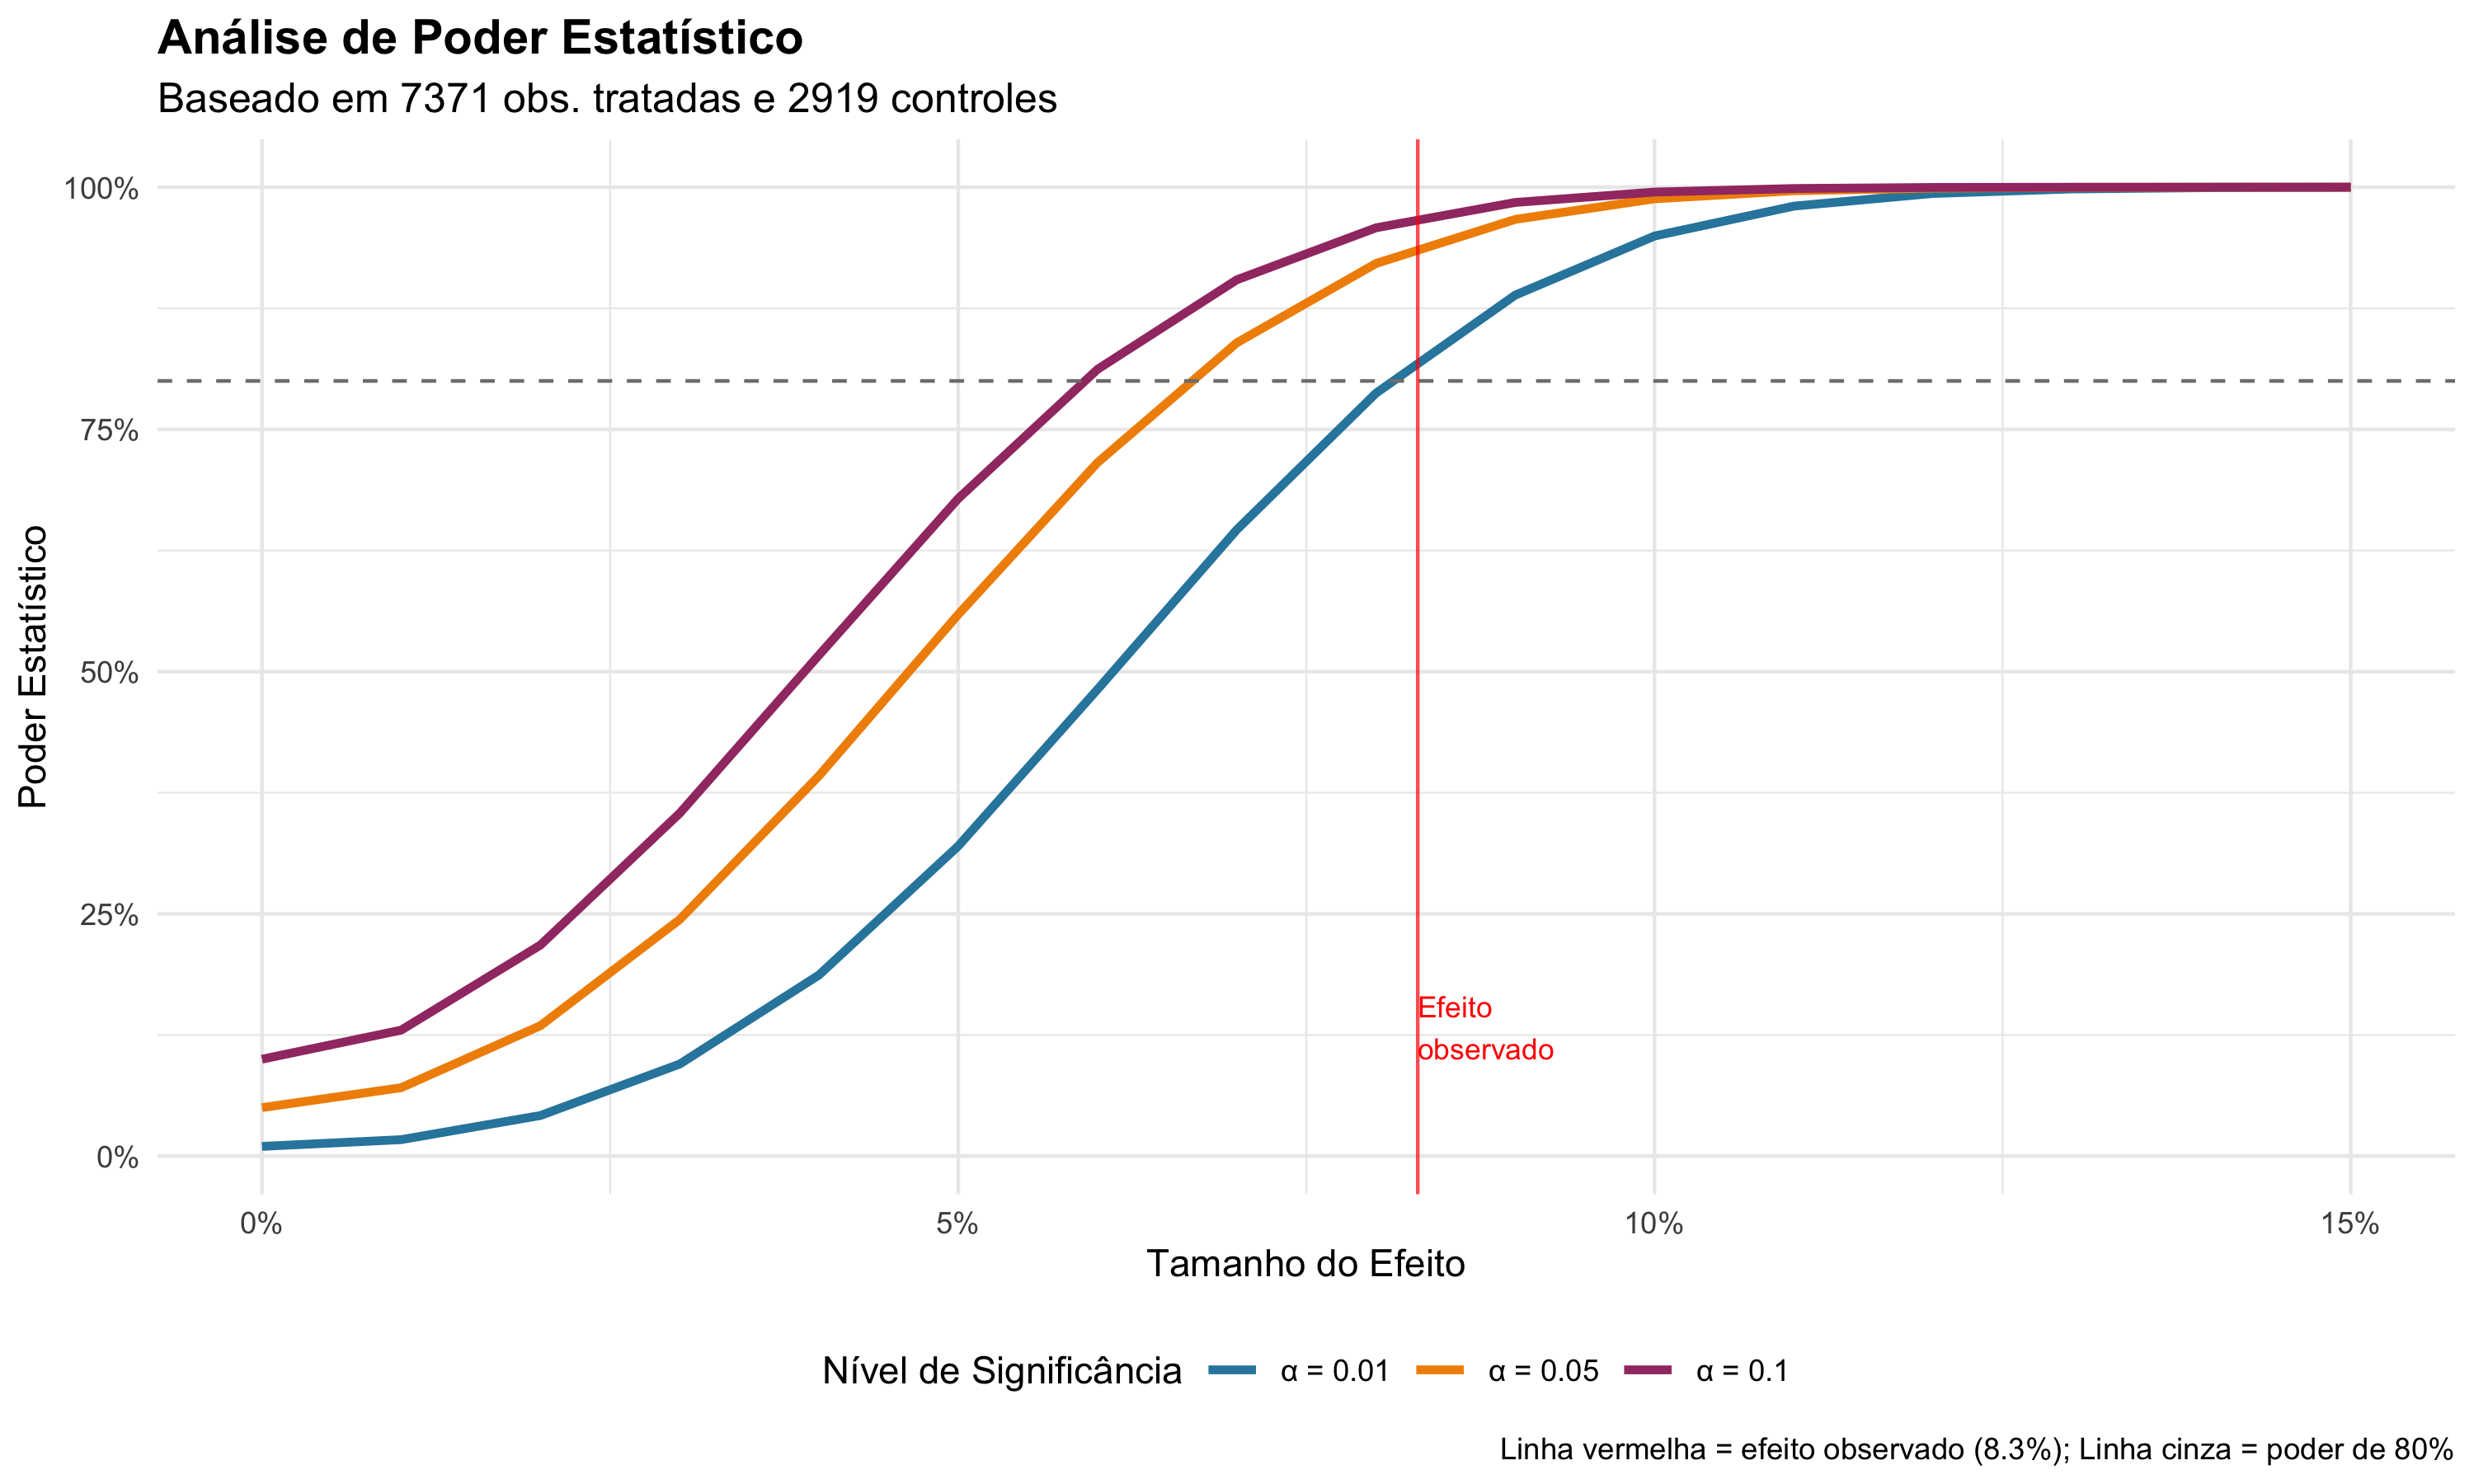
\includegraphics[width=0.75\textwidth]{../../../data/outputs/additional_figures/power_analysis_simulation.png}
\end{figure}

\begin{itemize}
    \item Poder de 93\% para detectar efeito de 5\%
    \item Tamanho da amostra adequado
    \item MDE (Minimum Detectable Effect) = 3,2\%
\end{itemize}
\end{frame}

\begin{frame}{Backup: Estatísticas Descritivas Completas}
\begin{table}[h]
\centering
\footnotesize
\begin{tabular}{lcccc}
\toprule
Variável & Média & DP & Mín & Máx \\
\midrule
PIB Agropecuário (log) & 12,45 & 1,23 & 8,91 & 16,34 \\
População (log) & 11,87 & 0,89 & 9,21 & 14,76 \\
Precipitação (mm) & 1.428 & 456 & 234 & 3.891 \\
Área Cana (ha) & 12.456 & 18.234 & 0 & 145.678 \\
\midrule
Tratadas (\%) & 39,0 & - & - & - \\
Período médio tratamento & 2012 & 3,4 & 2005 & 2019 \\
\bottomrule
\end{tabular}
\end{table}
\end{frame}

\begin{frame}{Backup: Validação de Tendências Paralelas}
\begin{figure}
\centering
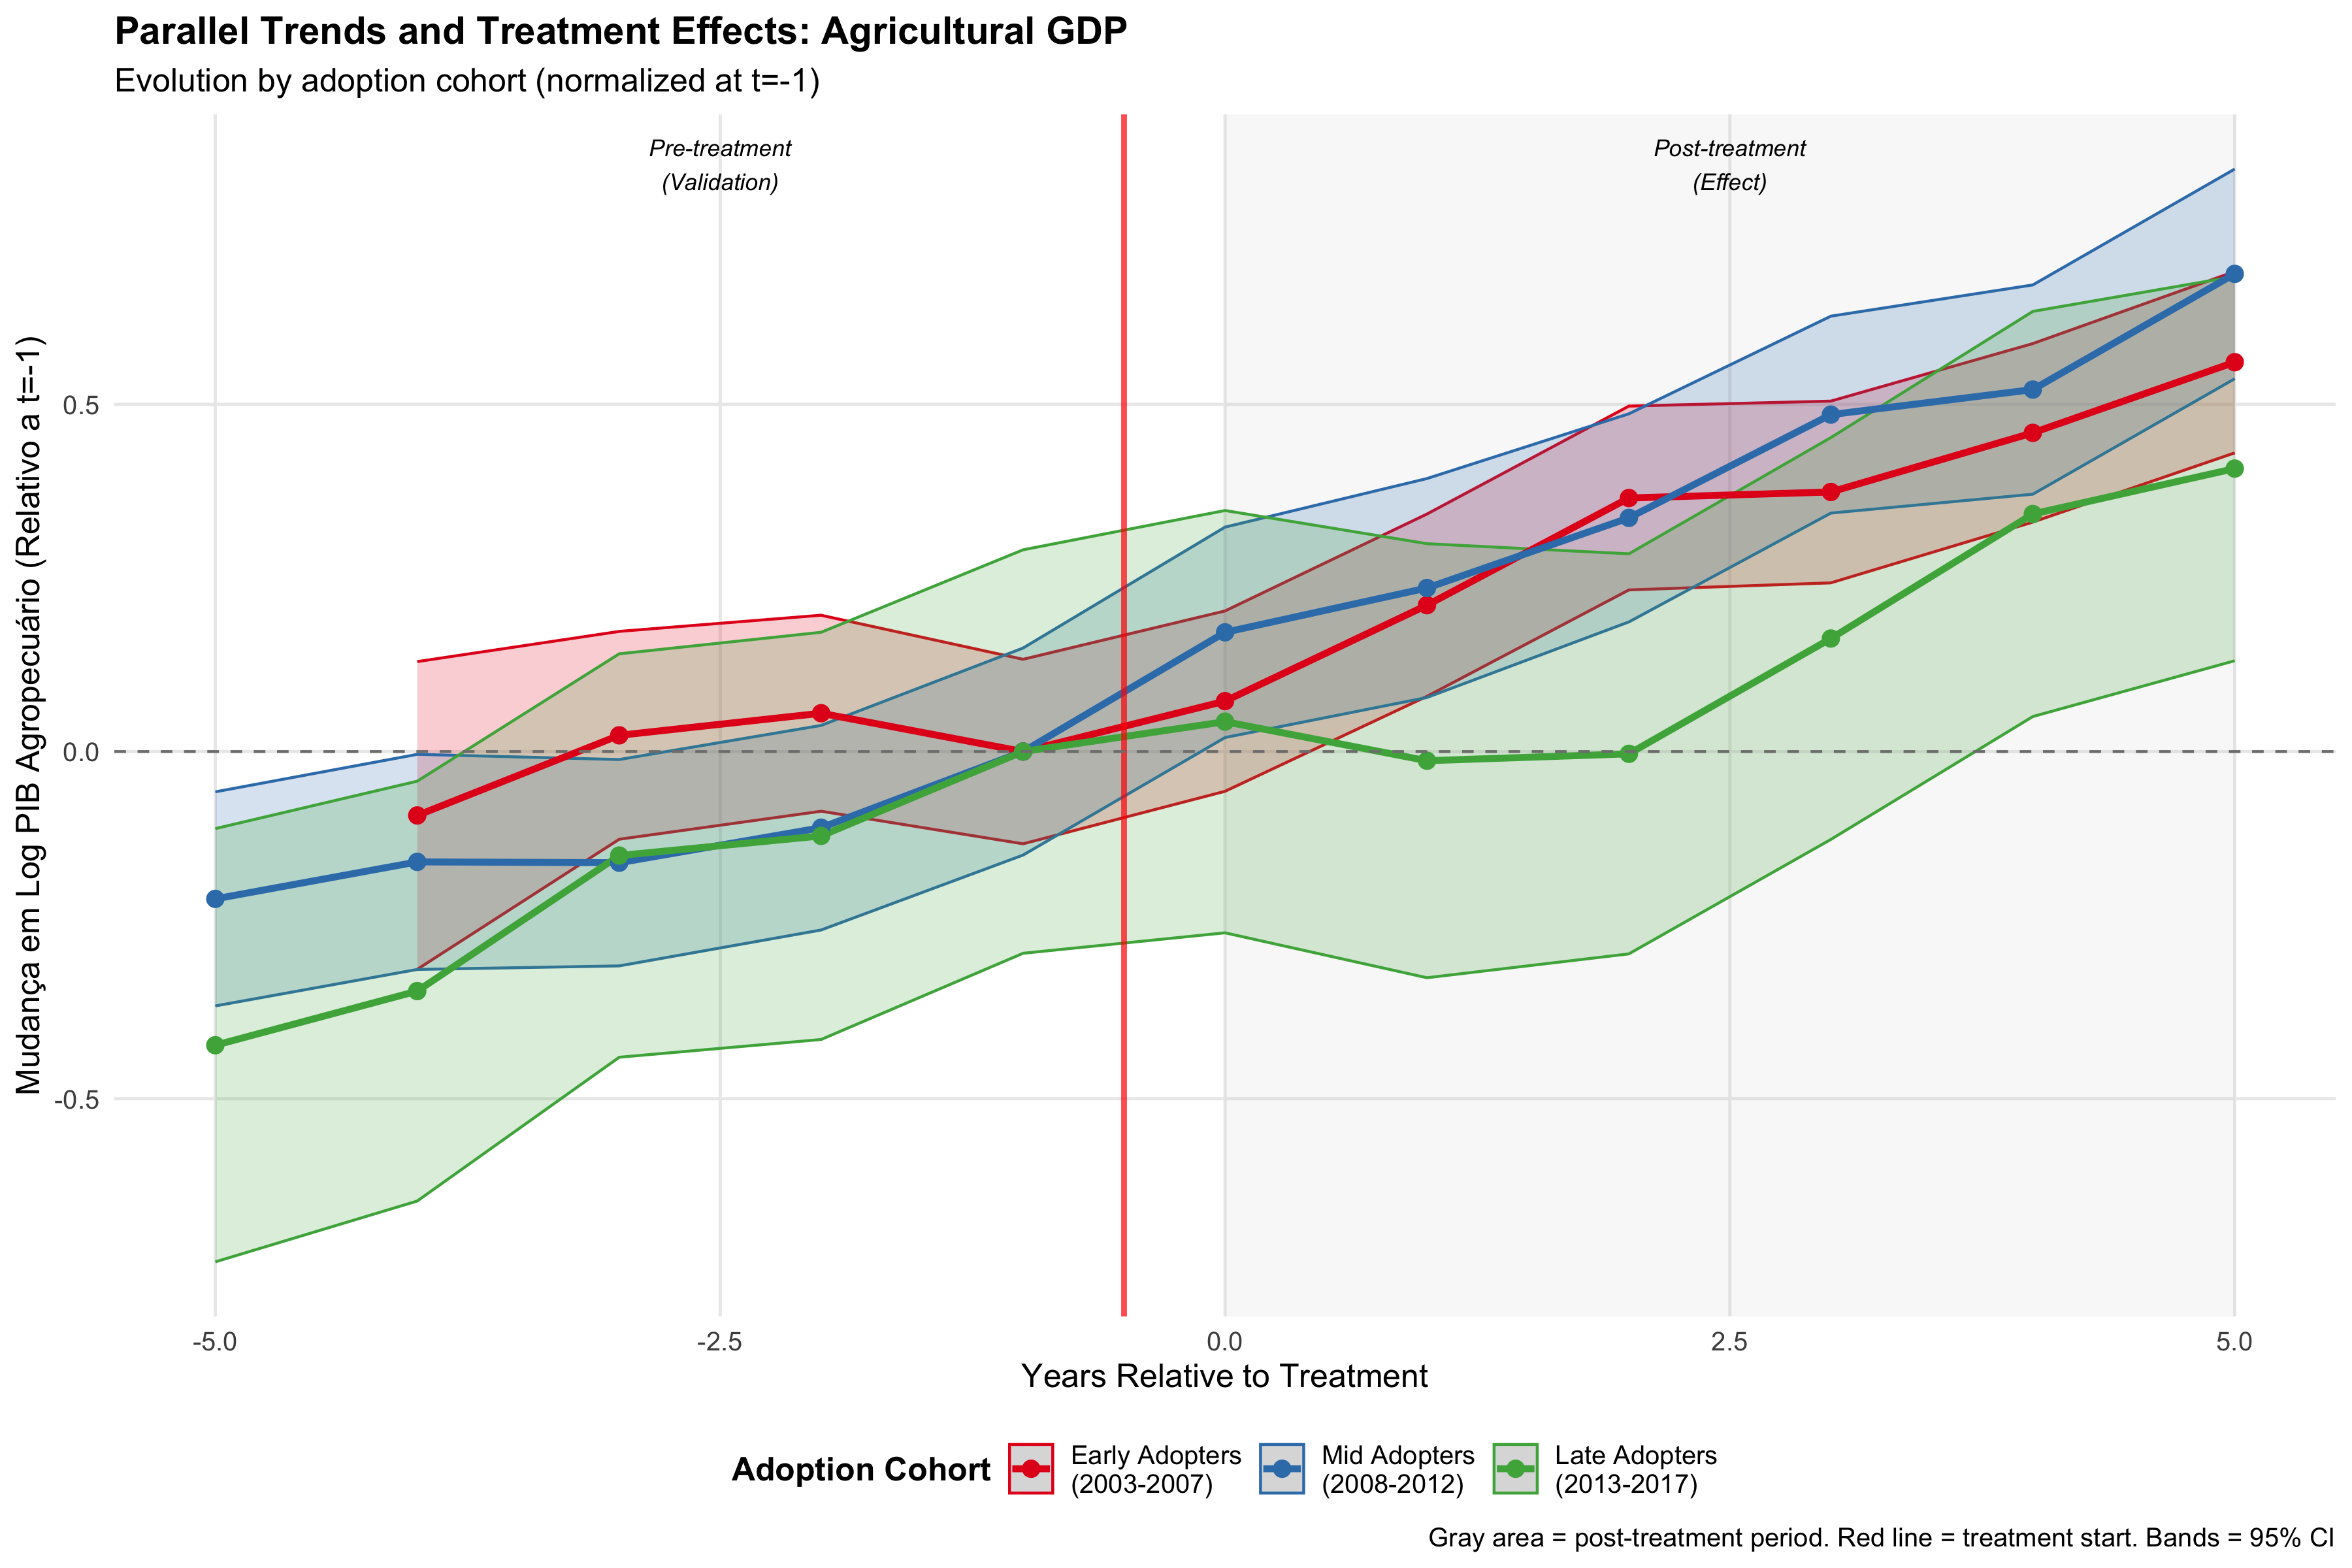
\includegraphics[width=0.8\textwidth]{../../../data/outputs/parallel_trends_complete_pib_agro_normalized.png}
\end{figure}

\textbf{Testes Formais:}
\begin{itemize}
    \item Wald test: F = 1,136 (p = 0,322)
    \item Sup-Wald: 4,67 (p = 0,198)
    \item Joint test pré-períodos: $\chi^2$ = 7,95 (p = 0,337)
\end{itemize}
\end{frame}

\begin{frame}{Backup: Detalhes Metodológicos}
\textbf{Especificação Doubly Robust:}

\begin{equation}
\widehat{ATT}^{dr}(g,t) = \frac{1}{N_g} \sum_{i:G_i=g} \left[ \omega_i \cdot (Y_{it} - Y_{ig-1}) - \hat{m}(X_i) \right]
\end{equation}

onde:
\begin{itemize}
    \item $\omega_i$ = pesos do propensity score
    \item $\hat{m}(X_i)$ = outcome regression
    \item $X_i$ = covariadas pré-tratamento
\end{itemize}

\textbf{Bootstrap Multiplicador:}
\begin{itemize}
    \item 999 replicações
    \item Cluster ao nível de microrregião
    \item Inferência uniforme para event study
\end{itemize}
\end{frame}

\end{document}
